\chapter{Πειραματική Αξιολόγηση}
\label{chap6}

\section{Εισαγωγή}
\label{chap6_Intro}

Για την αξιολόγηση της προτεινόμενης τεχνικής αντιμετώπισης των πλήρως ελαττωματικών συνόλων του Πίνακα Πρόβλεψης Προορισμού Διακλάδωσης εκτελέστηκαν εξομοιώσεις για 100 διαφορετικούς χάρτες σφαλμάτων και για όλα τα μετροπρογράμματα της σουίτας \spec. Επιπλέον, για κάθε περίπτωση χάρτη σφαλμάτων εκτελέστηκαν εξομοιώσεις για τρεις διαφορετικές παραλλαγές της τεχνικής. Στο παρόν κεφάλαιο παρουσιάζεται ο μέσος όρος των αποτελεσμάτων τους. Στο πρώτο τμήμα του κεφαλαίου μελετάται η βελτίωση της απόδοσης του υπερβαθμωτού επεξεργαστή όταν ενσωματώνεται η τεχνική της λογικής μετάθεσης πλαισίων στον Πίνακα Πρόβλεψης Προορισμού Διακλάδωσης. Στο δεύτερο τμήμα παρουσιάζονται τα αντίστοιχα αποτελέσματα ενέργειας ώστε να αποκαλυφθεί εάν η χρήση της προτεινόμενης τεχνικής επιφέρει ή όχι τη συνολική μείωση της κατανάλωσης του συστήματος.

%----------------------------------------------------------%

\section{Παράμετροι Αξιολόγησης}
\label{chap6_EvaluationParameters}

Η μελέτη που ακολουθεί επικεντρώνεται σε μνήμες των 2048 πλαισίων και δύο διαφορετικών μεγεθών οργάνωσης συνόλου συσχέτισης (τμήματα). Οι διαμορφώσεις αυτές αποτελούν μία μέση περίπτωση των σύγχρονων εμπορικών επεξεργαστών και για το λόγο αυτό μπορούν να θεωρηθούν αντικειμενικές. Όπως αναφέρθηκε και στην Ενότητα \ref{chap4_BTBConfigIPC}, ένας Πίνακας Πρόβλεψης Προορισμού Διακλάδωσης (ΠΠΠΔ) των 2048 πλαισίων έχει τη δυνατότητα να προσφέρει την απόδοση ακόμη και μίας εξαιρετικά μεγάλης μνήμης των 16384 πλαισίων.
\par
Για κάθε περίπτωση λειτουργίας χαμηλού δυναμικού εξετάζεται η μεταβολή της απόδοσης και της καταναλισκόμενης ενέργειας εξαιτίας της ύπαρξης ελαττωματικών κυψελίδων στον Πίνακα Πρόβλεψης Προορισμού Διακλάδωσης. Συγκεκριμένα μελετώνται οι δύο περιπτώσεις δυναμικού που αντιστοιχούν στις πιθανότητες σφάλματος $\expnum{2}$ (πιθανότητα-1) και $\expnum{5}$ (πιθανότητα-2).
\par
Σε κάθε περίπτωση εξομοιώθηκαν τέσσερα είδη μοντέλων Πίνακα Πρόβλεψης Προορισμού Διακλάδωσης. Το σύνολο των εξομοιώσεων που πραγματοποιήθηκαν για κάθε χάρτη σφαλμάτων και μετροπρόγραμμα παρουσιάζονται στον Πίνακα \ref{tab:chap6_LowPowerSimulations}.

\begin{table}[t]
    \centering
    \begin{tabularx}{\textwidth}{!{\vrule width 4\arrayrulewidth} >{\centering\arraybackslash}X | >{\centering\arraybackslash}X | >{\centering\arraybackslash}X !{\vrule width 4\arrayrulewidth}}
        \Xhline{4\arrayrulewidth}
        \textbf{Μοντέλο ΠΠΠΔ}   & \textbf{Οργάνωση ΠΠΠΔ}                 & \textbf{Πιθανότητα Σφάλματος (Συχνότητα)} \\
        \Xhline{4\arrayrulewidth}
        
        \multirow{4}{*}{Βασικό} & \multirow{2}{*}{2048-πλαίσια/2-τρόπων} & {$\expnum{2}\ (1.1GHz)$} \\ \cline{3-3}
                                &                                        & {$\expnum{5}\ (0.5GHz)$} \\ \cline{2-3}
                                & \multirow{2}{*}{2048-πλαίσια/4-τρόπων} & {$\expnum{2}\ (1.1GHz)$} \\ \cline{3-3}
                                &                                        & {$\expnum{5}\ (0.5GHz)$} \\
        \hline
        
        \multirow{4}{\linewidth}{\centering Ενισχυμένο Σειριακό} & \multirow{2}{*}{2048-πλαίσια/2-τρόπων} & {$\expnum{2}\ (1.1GHz)$} \\ \cline{3-3}
                                                                 &                                        & {$\expnum{5}\ (0.5GHz)$} \\ \cline{2-3}
                                                                 & \multirow{2}{*}{2048-πλαίσια/4-τρόπων} & {$\expnum{2}\ (1.1GHz)$} \\ \cline{3-3}
                                                                 &                                        & {$\expnum{5}\ (0.5GHz)$} \\
        \hline
        
        \multirow{4}{\linewidth}{\centering Ενισχυμένο Παράλληλο} & \multirow{4}{*}{2048-πλαίσια/4-τρόπων} & \multirow{2}{*}{$\expnum{2}\ (1.1GHz)$} \\
                                                                  &                                        &                          \\ \cline{3-3}
                                                                  &                                        & \multirow{2}{*}{$\expnum{5}\ (0.5GHz)$} \\
                                                                  &                                        &                          \\
        \hline
        
        \multirow{4}{\linewidth}{\centering Βελτιστοποιημένο Σειριακό} & \multirow{2}{*}{2048-πλαίσια/2-τρόπων} & {$\expnum{2}\ (1.1GHz)$} \\ \cline{3-3}
                                                                          &                                        & {$\expnum{5}\ (0.5GHz)$} \\ \cline{2-3}
                                                                          & \multirow{2}{*}{2048-πλαίσια/4-τρόπων} & {$\expnum{2}\ (1.1GHz)$} \\ \cline{3-3}
                                                                          &                                        & {$\expnum{5}\ (0.5GHz)$} \\
        \hline
        
        \hline
        \textbf{Σύνολο Εξομοιώσεων} & \multicolumn{2}{c !{\vrule width 4\arrayrulewidth}}{14 $\times$ 29 μετροπρογράμματα $\times$ 100 χάρτες σφ. = \textbf{40600}} \\
        \Xhline{4\arrayrulewidth}
    \end{tabularx}
    \caption{Εκτελούμενες εξομοιώσεις σε λειτουργία χαμηλής κατανάλωσης}
    \label{tab:chap6_LowPowerSimulations}
\end{table}

Για κάθε ένα από τα τέσσερα εξομοιούμενα μοντέλα που παρουσιάζονται στον Πίνακα \ref{tab:chap6_LowPowerSimulations} ισχύουν οι ακόλουθες παραδοχές:
\begin{description}
    \item[Βασικό:] Απενεργοποίηση όλων των ελαττωματικών πλαισίων.
    \item[Ενισχυμένο Σειριακό:] Απενεργοποίηση όλων των ελαττωματικών πλαισίων και λογική μετάθεση τους με τη χρήση ενός καταχωρητή ανά τμήμα. Η εύρεση κατάλληλων τιμών προκύπτει από την εκτέλεση του σειριακού αλγορίθμου.
    \item[Ενισχυμένο Παράλληλο:] Απενεργοποίηση όλων των ελαττωματικών πλαισίων και λογική μετάθεση τους με τη χρήση ενός καταχωρητή ανά τμήμα. Η εύρεση κατάλληλων τιμών προκύπτει από την εκτέλεση του παράλληλου αλγορίθμου.
    \item[Βελτιστοποιημένο Σειριακό:] Απενεργοποίηση όλων των ελαττωματικών πλαισίων και λογική μετάθεση τους με τη χρήση πολλαπλών καταχωρητών ανά τμήμα. Η εύρεση κατάλληλων τιμών προκύπτει από την εκτέλεση του σειριακού αλγορίθμου.
\end{description}

%----------------------------------------------------------%

\section{Σύστημα Αξιολόγησης}
\label{chap6_EvaluationSystem}

Για την αξιολόγηση της τεχνικής χρησιμοποιήθηκες ο το μαθηματικό εργαλείο \matlab για την εξαγωγή των 100 χαρτών σφαλμάτων, σε συνδυασμό με τον εγκεκριμένο εξομοιωτή αρχιτεκτονικής υπολογιστών \gem. Επιπλέον, χρησιμοποιήθηκε το εργαλείο υπολογισμού κατανάλωσης \mcpat το οποίο δέχεται ως είσοδο τα αποτελέσματα της εξομοίωσης. Για τον υπολογισμό της ισχύος του Πίνακα Πρόβλεψης Προορισμού Διακλάδωσης και αξιοποιεί το εργαλείο \cacti, το οποίο ενσωματώνεται στον πηγαίο του κώδικα. Αναλυτικές πληροφορίες για τα τρία αυτά εργαλεία βρίσκονται στα \cite{release2013mathworks}, \cite{binkert2011gem5} και \cite{li2009mcpat, muralimanohar2009cacti} αντίστοιχα. Στο Κεφάλαιο \ref{chap7} γίνεται λεπτομερής περιγραφή της διαδικασία αξιολόγησης και του τρόπου χρήσης των εργαλείων.
\par
Στον Πίνακα \ref{tab:chap6_gem5parameters} παρουσιάζονται οι λεπτομέρειες του εξομοιούμενου \en{x86} επεξεργαστή που χρησιμοποιήθηκε κατά την εκτέλεση των πειραμάτων, καθώς και επιπλέον πληροφορίες για τα μετροπρογράμματα που χρησιμοποιήθηκαν.

\begin{otherlanguage}{english}
    \begin{table}[h]
        \centering
        \begin{tabularx}{\textwidth}{ >{\centering\arraybackslash}X || >{\centering\arraybackslash}X }
            
            \Xhline{4\arrayrulewidth}
            
            \textbf{\gr{Παράμετροι}}                                        & \textbf{\gr{Τιμές}}                \\
            
            \Xhline{4\arrayrulewidth}
            
            CPU Architecture / ISA                                          & Out of Order / x86                 \\ \hline
            
            ROB/IQ/LQ/SQ/Registers                                          & 256/128/128/128/256                \\ \hline
            
            Pipeline Depth                                                  & 10                                 \\ \hline
            
            Fetch/Issue/Commit Width                                        & 8/8/8 Instructions Per Cycle       \\ \hline
            
            {}                                                              & Local History Table: 4k-entries,   \\
            Combined Branch Predictor                                       & Local Predictor: 4k-entries,       \\
            (Tournament Predictor)                                          & Global Predictor: 16k-entries,     \\
            {}                                                              & Choice Predictor: 16k-entries      \\ \hline
            
            Branch Target Buffer                                            & 2048-entries, 2-way/4-way          \\ \hline
            
            \multirow{2}{*}{L1 Instruction \& L1 Data Caches}               & 64kB, 8-way, 64B-block, 1-cycle,   \\
                                                                            & LRU, MSHRS, Write Buffers          \\ \hline
                                                                
            \multirow{2}{*}{L2 Cache}                                       & 8MB, 32-way, 64B-block, 15-cycles, \\
                                                                            & LRU, 40 MSHRS, Write Buffers       \\ \hline
            
            Stride Prefetcher (L2 Cache)                                    & PC-indexed, 128-entries 8-degree   \\ \hline
            
            DRAM                                                            & 2GB, 60ns, 12.8GB/s                \\ \hline
            
            Process Technology                                              & 22nm SOI                           \\ \hline
            
            Nominal Operation                                               & 2.5GHz, 1Volt                      \\ \hline
            
            Studied SRAM                                                    & pfail1: 2e-03 (1.1GHz, 0.47Volts)  \\ \cline{2-2}
            Probabilities of Failures (pfails) \cite{lorente2014analyzing}  & pfail2: 5e-03 (0.5GHz, 0.42Volts)  \\ \hline
            
            \multirow{2}{*}{\spec Benchmarks \cite{henning2006spec}}        & 17 Floating Point (SPECfp2006)     \\
                                                                            & 12 Integer (SPECint2006)           \\ \hline
            
            Simulated Instructions                                          & 3B Warm-up, 500M Committed         \\ \hline
            
            \Xhline{4\arrayrulewidth}
        \end{tabularx}
        \caption{\gr{Παράμετροι εξομοιωτή} \gem}
        \label{tab:chap6_gem5parameters}
    \end{table}
\end{otherlanguage}

%----------------------------------------------------------%

\section{Αποτελέσματα \gem}
\label{chap6_gem5Results}

Στην παρούσα ενότητα αναδεικνύεται η βελτίωση που προσφέρει η μελετώμενη τεχνική (ενισχυμένο/βελτιστοποιημένο μοντέλο) στο χρόνο εκτέλεσης ενός προγράμματος (Εντολές ανά Κύκλο Ρολογιού - \ipc), συγκριτικά με την απλή απενεργοποίηση των ελαττωματικών πλαισίων (βασικό μοντέλο). Στην πρώτη υποενότητα μελετάται η περίπτωση όπου κάθε τμήμα του Πίνακα Πρόβλεψης Προορισμού Διακλάδωσης (ΠΠΠΔ) περιέχει έναν καταχωρητή διαμόρφωσης και για τον υπολογισμό τιμών χρησιμοποιείται ο σειριακός αλγόριθμος. Στη δεύτερη υποενότητα μελετάται η περίπτωση όπου ο υπολογισμός τιμών των καταχωρητών γίνεται μέσω του παράλληλου αλγορίθμου. Στη τρίτη και τελευταία υποενότητα μελετάται η περίπτωσης όπου τα τμήματα του Πίνακα Πρόβλεψης Προορισμού Διακλάδωσης χωρίζονται σε υποτμήματα με ένα ξεχωριστό Καταχωρητή Διαμόρφωσης για κάθε ένα, οι τιμές των οποίων υπολογίζονται μέσω του σειριακού αλγορίθμου.
\par
Για την περίπτωση του βελτιστοποιημένου μοντέλου χρησιμοποιήθηκε ένα μέσο πλήθος καταχωρητών ανά τμήμα για κάθε οργάνωση ώστε να επιτυγχάνεται η κατά το δυνατόν μεγαλύτερη μείωση των πλήρως ελαττωματικών συνόλων σε όλες τις περιπτώσεις τάσεων λειτουργίας. Σύμφωνα με τα αποτελέσματα του μέσου όρου 1000 χαρτών που μελετήθηκαν στην Ενότητα \ref{chap5_AlgorithmResults} και τα οποία επισημαίνονται στο Σχήμα \ref{fig:chap6_btb_ffsets_2048}, για την οργάνωση 2-τρόπων η επιλογή 64 καταχωρητών ανά τμήμα αποτελεί μία ικανοποιητική επιλογή ώστε να επιτυγχάνεται σημαντική μείωση των πλήρως ελαττωματικών συνόλων σε συνδυασμό με ένα σχετικά μικρό κόστος. Αντίστοιχα, για την οργάνωση 4-τρόπων η χρήση 4 καταχωρητών σε συνδυασμό με την εκτέλεση του σειριακού αλγορίθμου για τον υπολογισμό τιμών τους, οδηγεί σε ολοκληρωτική απαλοιφή τους με ελάχιστη αύξηση του κόστους.
\par
Οι γραφικές παραστάσεις που ακολουθούν απεικονίζουν τη μείωση που υφίσταται η απόδοση του υπερβαθμωτού επεξεργαστή όταν στον Πίνακα Πρόβλεψης Προορισμού Διακλάδωσης υπάρχουν ελαττωματικά πλαίσια σε σχέση με την περίπτωση όπου εφαρμόζεται κανονική τάση δυναμικού με την ίδια συχνότητα λειτουργίας, οι οποίες αναφέρθηκαν στον Πίνακα \ref{tab:chap4_NominalSimulations}.

\begin{figure}[!b]
    \centering
    \begin{subfigure}[t]{0.5\textwidth}
        \centering
        \fbox{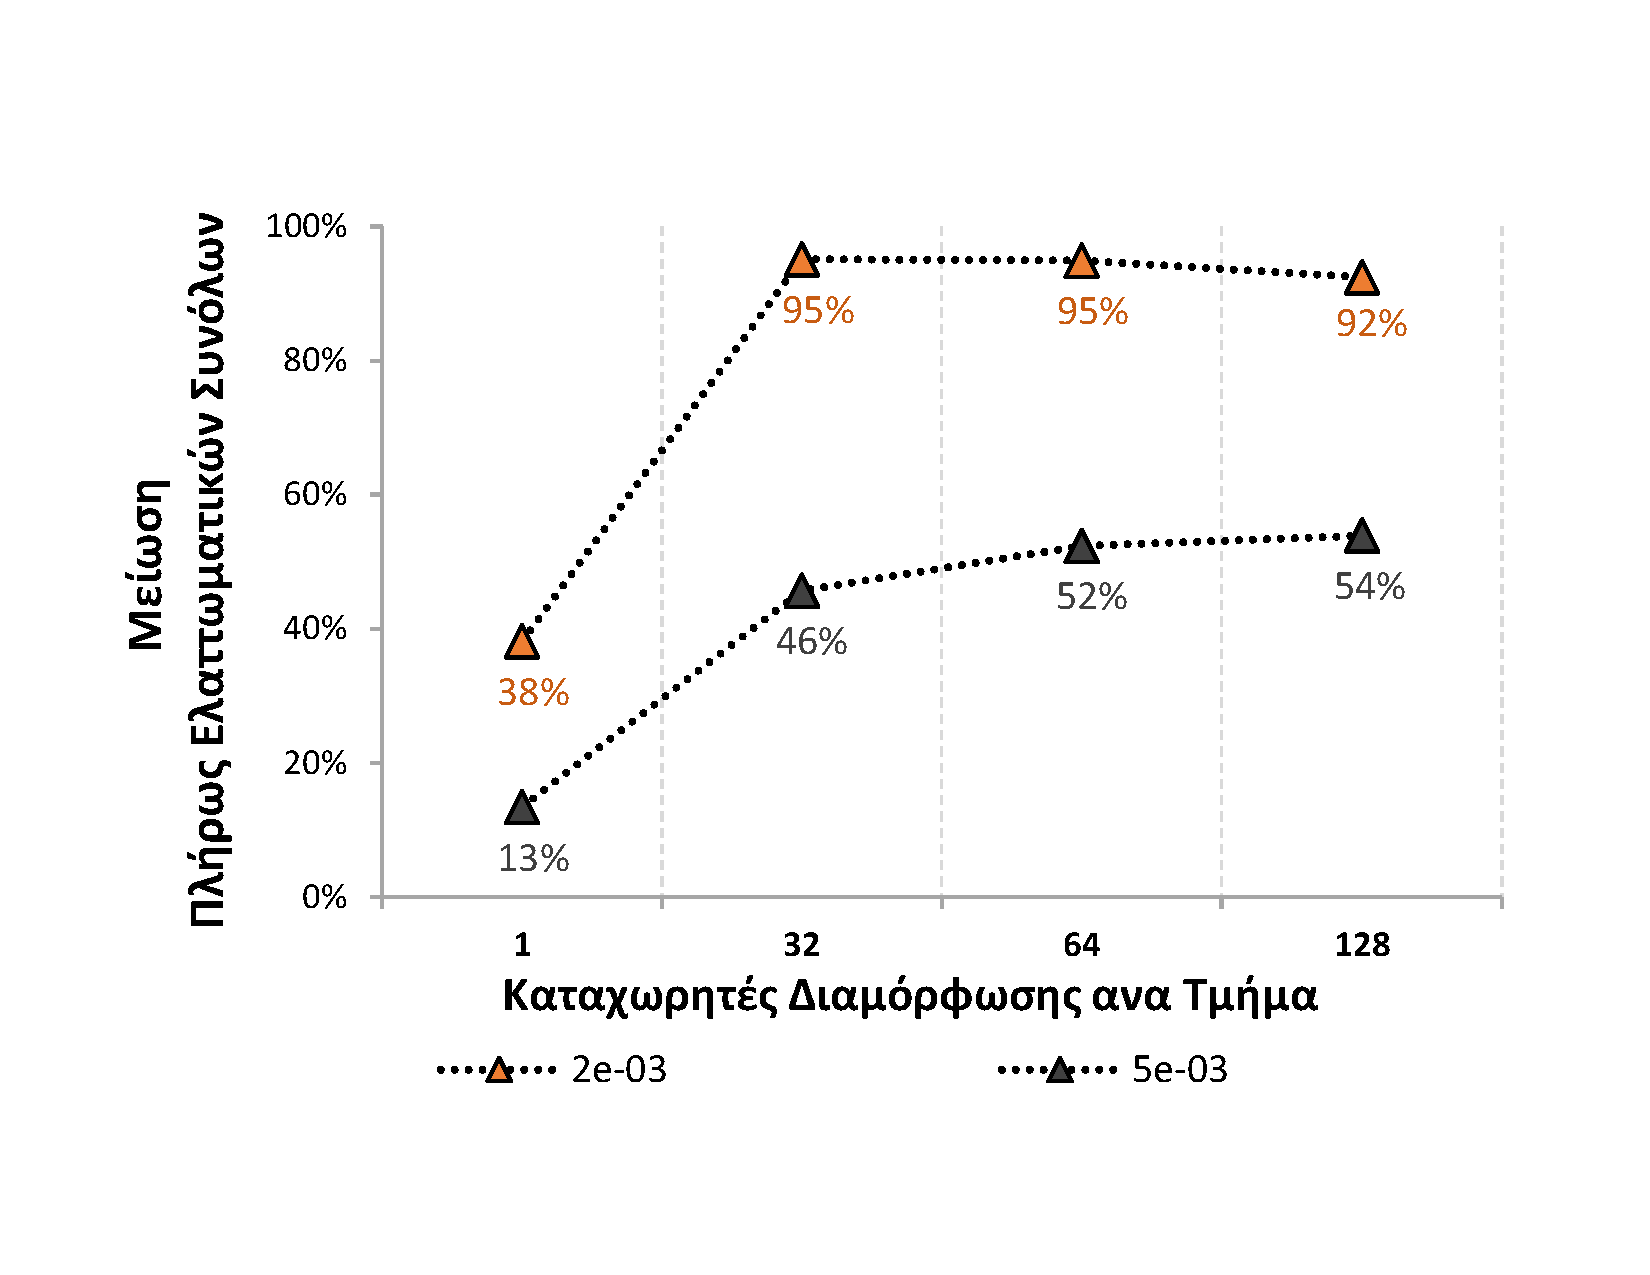
\includegraphics[width=0.99\linewidth, trim=2cm 2.9cm 1.8cm 3.5cm, clip=true]{\resultsDIR/chap6_BTB_ffsets_reduction_2048_2way.pdf}}
        \caption{ΠΠΠΔ 2048-πλαισίων/2-τρόπων}
        \label{fig:chap6_btb_ffsets_2048_2way}
    \end{subfigure}%
    \begin{subfigure}[t]{0.5\textwidth}
        \centering
        \fbox{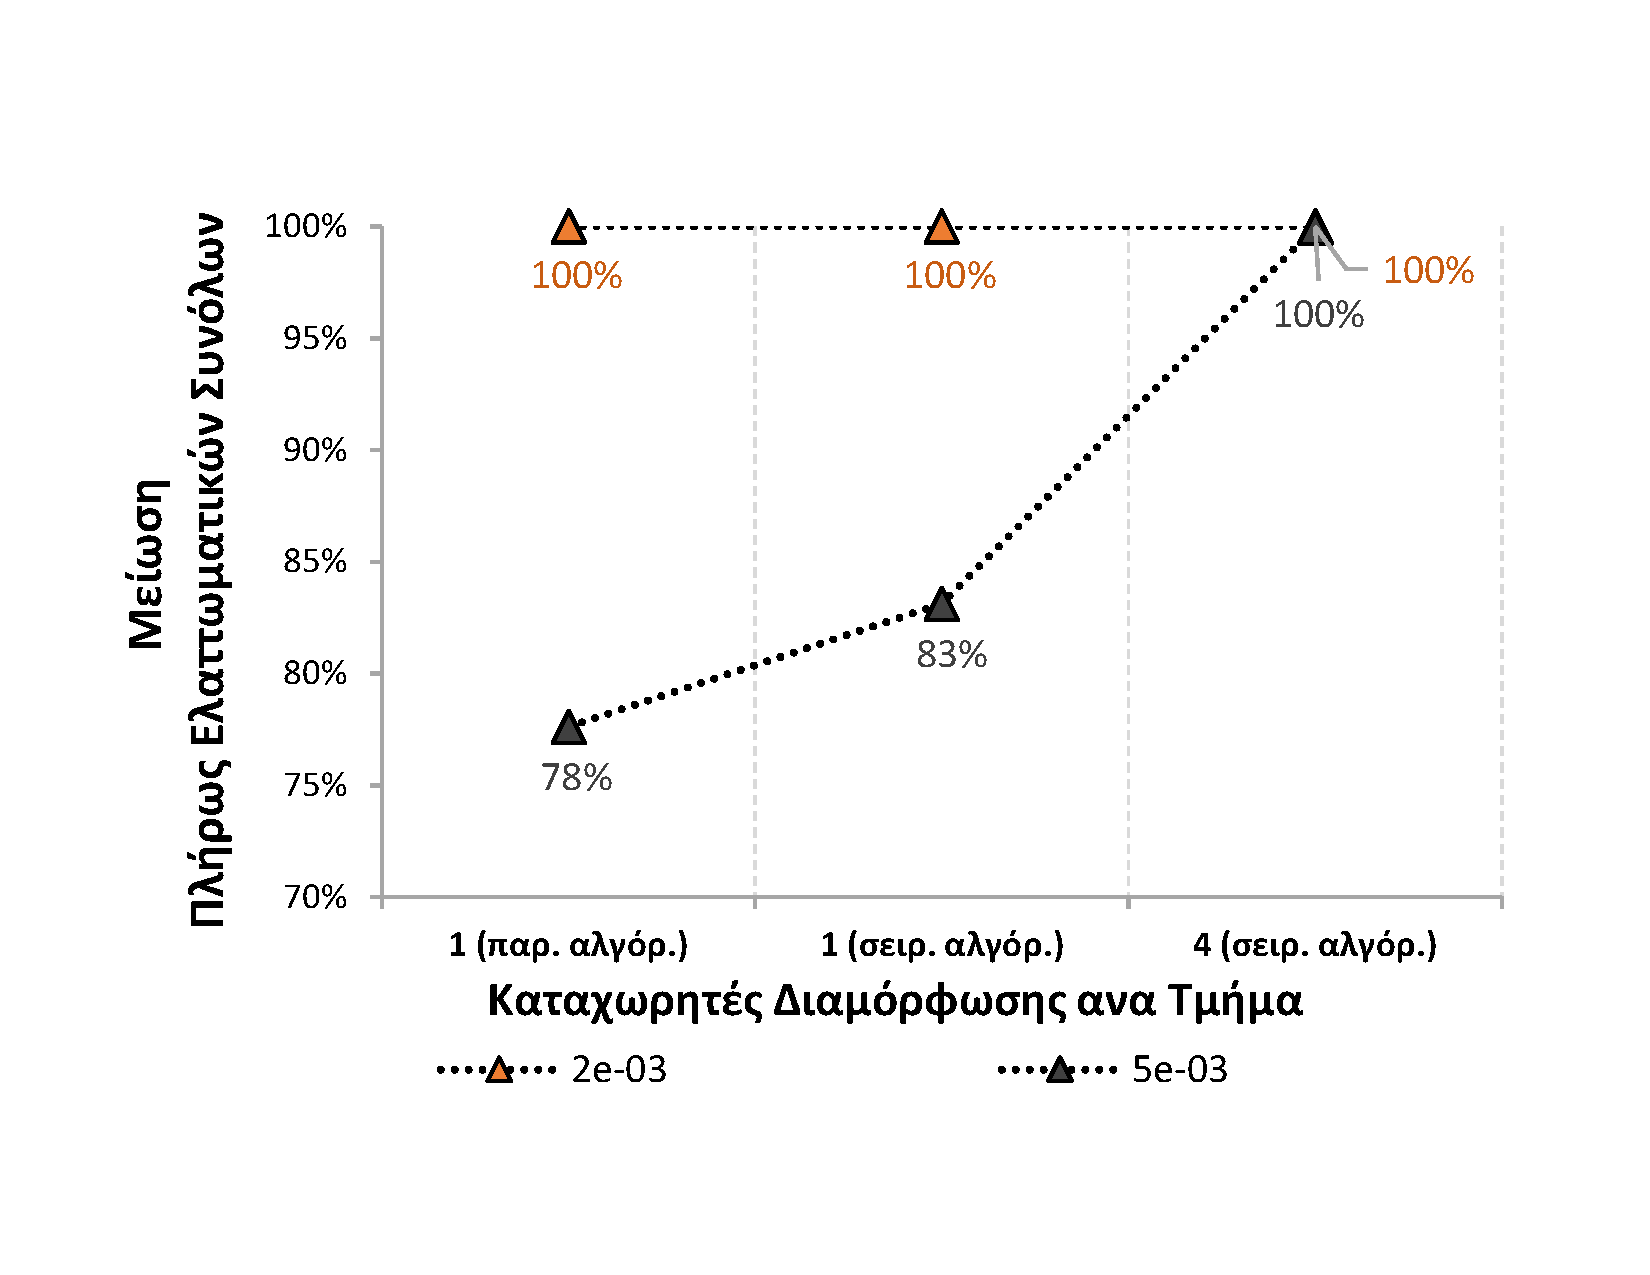
\includegraphics[width=0.99\linewidth, trim=2cm 2.9cm 1.8cm 3.5cm, clip=true]{\resultsDIR/chap6_BTB_ffsets_reduction_2048_4way.pdf}}
        \caption{ΠΠΠΔ 2048-πλαισίων/4-τρόπων}
        \label{fig:chap6_btb_ffsets_2048_4way}
    \end{subfigure}
    \caption{Μείωση των πλήρως ελαττωματικών πλαισίων με τη χρήση των προτεινόμενων μοντέλων ως προς το βασικό μοντέλο (υποπεριπτώσεις του Σχήματος \ref{fig:chap5_btb_ffsets_2048})}
    \label{fig:chap6_btb_ffsets_2048}
\end{figure}

Η μείωση της απόδοσης ισοδυναμεί με τη μείωση του ρυθμού ολοκλήρωσης εντολών (\ipc) η οποία υπολογίζεται από την εξίσωση:

\begin{equation}
    \label{eqn:chap6_IPCfaulty}
    \mathgr{Μείωση}\_IPC = \frac{IPC_\mathgr{χωρίς\_σφάλματα} - IPC_\mathgr{εξομοιούμενο\_μοντέλο\_με\_σφάλματα}}{IPC_\mathgr{χωρίς\_σφάλματα}}
\end{equation}

Τα αποτελέσματα αποτελούν τη μέση τιμή των 100 διαφορετικών εξομοιώσεων χαρτών σφαλμάτων. Το ποσοστό 0\% αντιστοιχεί σε μηδενική απώλεια απόδοσης (\ipc με σφάλματα στον Πίνακα Πρόβλεψης Προορισμού Διακλάδωσης = \ipc χωρίς σφάλματα στον Πίνακα Πρόβλεψης Προορισμού Διακλάδωσης) ενώ το ποσοστό 100\% ισοδυναμεί σε ολοκληρωτική απώλεια της απόδοσης (αδυναμία εκτέλεσης του προγράμματος). Η μεταβολή της απόδοσης παρουσιάζεται ξεχωριστά για κάθε μετροπρόγραμμα διότι η Μονάδα Δυναμικής Πρόβλεψης Διακλαδώσεων κατέχει διαφορετική βαρύτητα στο χρόνο εκτέλεσής τους. Τέλος, σε όλα τα γραφήματα της παρούσας ενότητας οι μπάρες κόκκινων αποχρώσεων αντιστοιχούν στα αποτελέσματα του βασικού μοντέλου ενώ οι μπάρες πράσινων αποχρώσεων σε αυτά του ενισχυμένου/βελτιστοποιημένου. Οι μελετώμενες πιθανότητες σφάλματος σε κάθε περίπτωση είναι $\expnum{2}$ και $\expnum{5}$ (Πιθανότητα Σφάλματος 1 και Πιθανότητα Σφάλματος 2 αντίστοιχα).

%----------------------------------------------------------%

\subsection{Αποτελέσματα Ενισχυμένου Σειριακού Μοντέλου}
\label{chap6_gem5SerialAlgResults}

Στα ακόλουθα γραφήματα παρουσιάζεται η σύγκριση μεταξύ βασικού και ενισχυμένου μοντέλου, όταν γίνεται χρήση του σειριακού αλγόριθμος. Όπως αναφέρεται και στον Πίνακα \ref{tab:chap6_LowPowerSimulations}, πραγματοποιήθηκαν εξομοιώσεις για οργανώσεις 2 και 4-τρόπων συνόλου συσχέτισης.
\par
Τα γραφήματα του Σχήματος \ref{fig:chap6_serial_2way_ipc} αναφέρονται τις περιπτώσεις Πίνακα Πρόβλεψης Προορισμού Διακλάδωσης 2-τρόπων. Όπως αναγράφεται στο πρώτο γράφημα \ref{fig:chap6_serial_2way_pail1_ipc}, στην πιθανότητα σφάλματος $\expnum{2}$, όπου τα ελαττωματικά πλαίσια αποτελούν το $19\%$ των συνολικών πλαισίων, η μείωση που υφίσταται ο ρυθμός ολοκλήρωσης εντολών (\ipc) εξαιτίας των σφαλμάτων στον Πίνακα Πρόβλεψης Προορισμού Διακλάδωσης ελαττώνεται κατά μέσο όρο από $8.6\%$ σε $5.9\%$. Επομένως, η τεχνική της λογικής μετάθεσης πλαισίων με τη χρήση ενός καταχωρητή ανά τμήμα σε συνδυασμό με τη χρήση του σειριακού αλγορίθμου, κατά μέσο όρο μπορεί να επαναφέρει το $32\%$ της απώλειας απόδοσης. Σε ορισμένες περιπτώσεις μετροπρογραμμάτων η βελτίωση που προσφέρει η τεχνική είναι ακόμα μεγαλύτερου μεγέθους, όπως για παράδειγμα στο \en{hmmer} όπου η μείωση της απόδοσης μεταβάλλεται από $9.9\%$ σε $3.1\%$ (επαναφορά κατά $68\%$).

\begin{figure}[!t]
    \centering
    \begin{subfigure}[t]{\textwidth}
        \centering
        \fbox{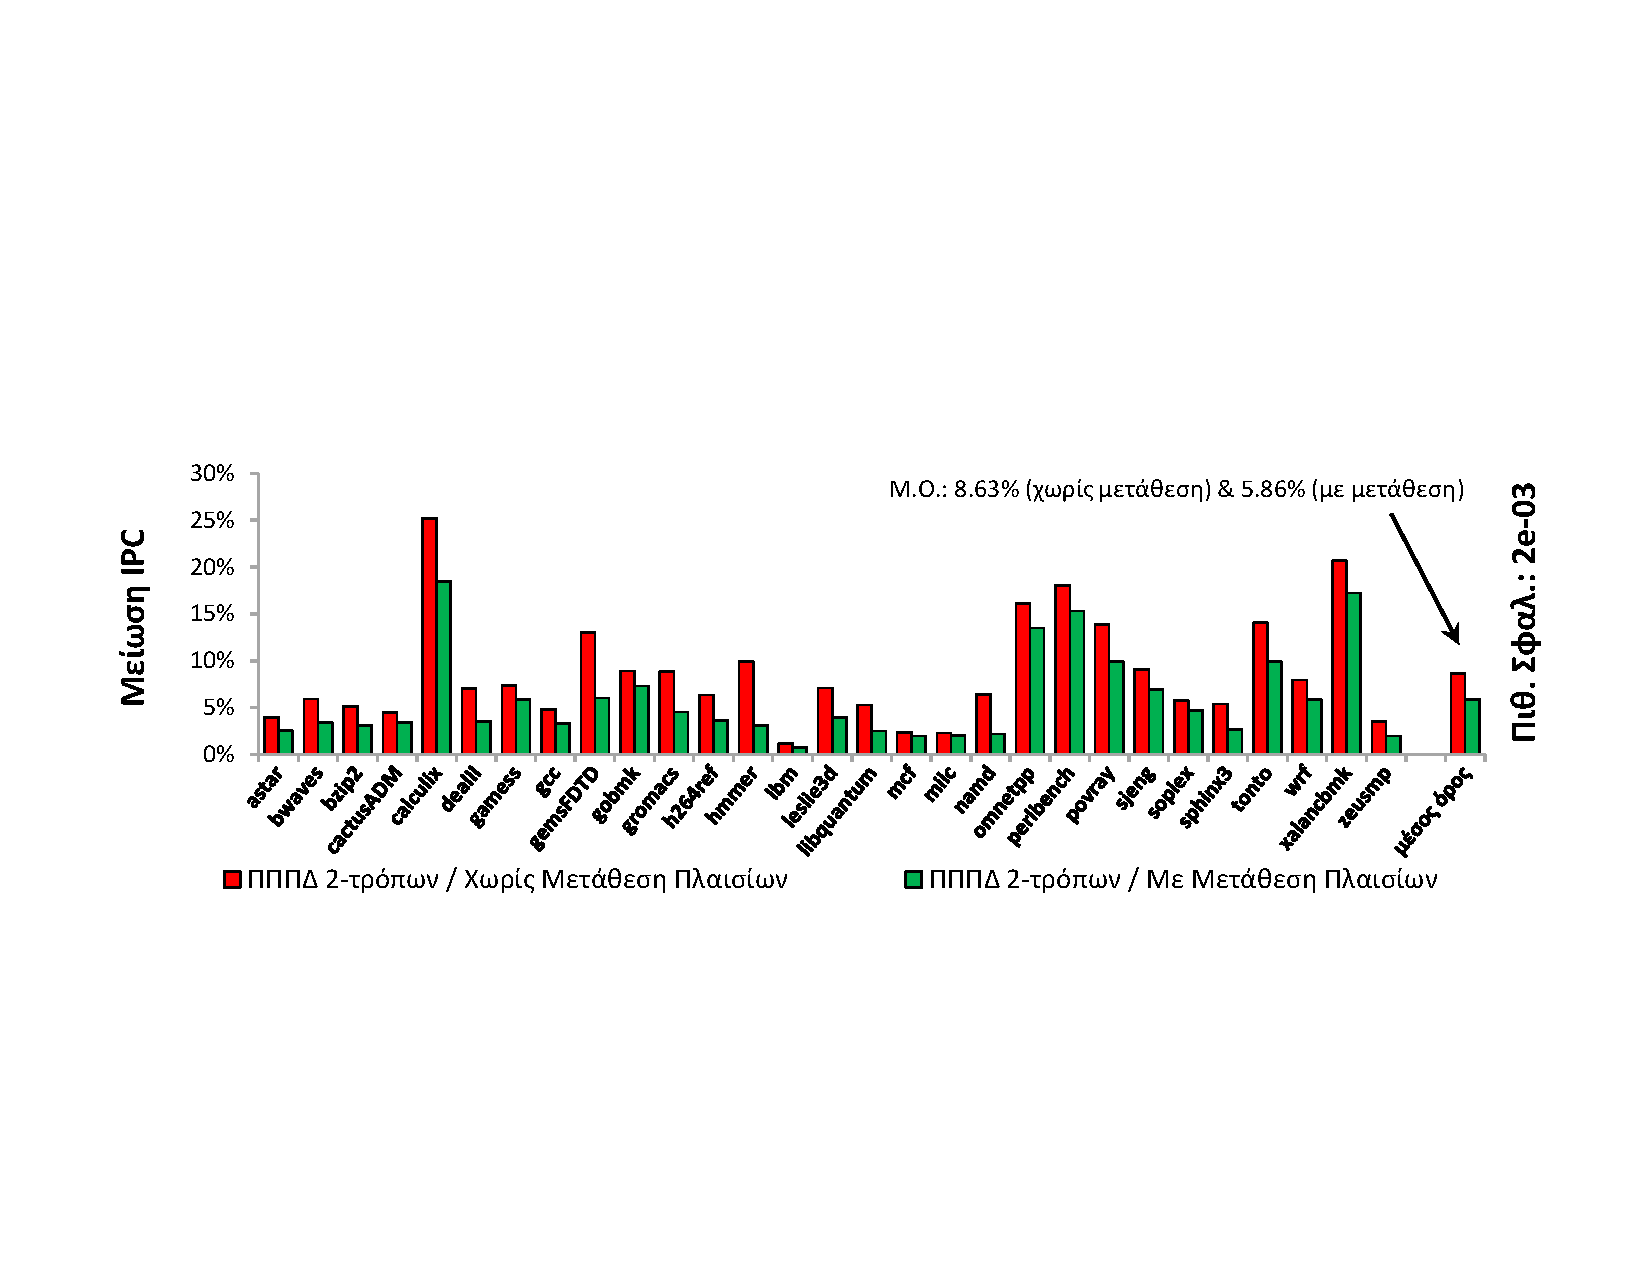
\includegraphics[width=\linewidth, trim=2cm 6.4cm 1.6cm 7.8cm, clip=true]{\resultsDIR/chap6_BTB_ipc_serial_w2_pfail1.pdf}}
        \caption{Πιθανότητα Σφάλματος 1}
        \label{fig:chap6_serial_2way_pail1_ipc}
    \end{subfigure}
    
    \begin{subfigure}[t]{\textwidth}
        \centering
        \fbox{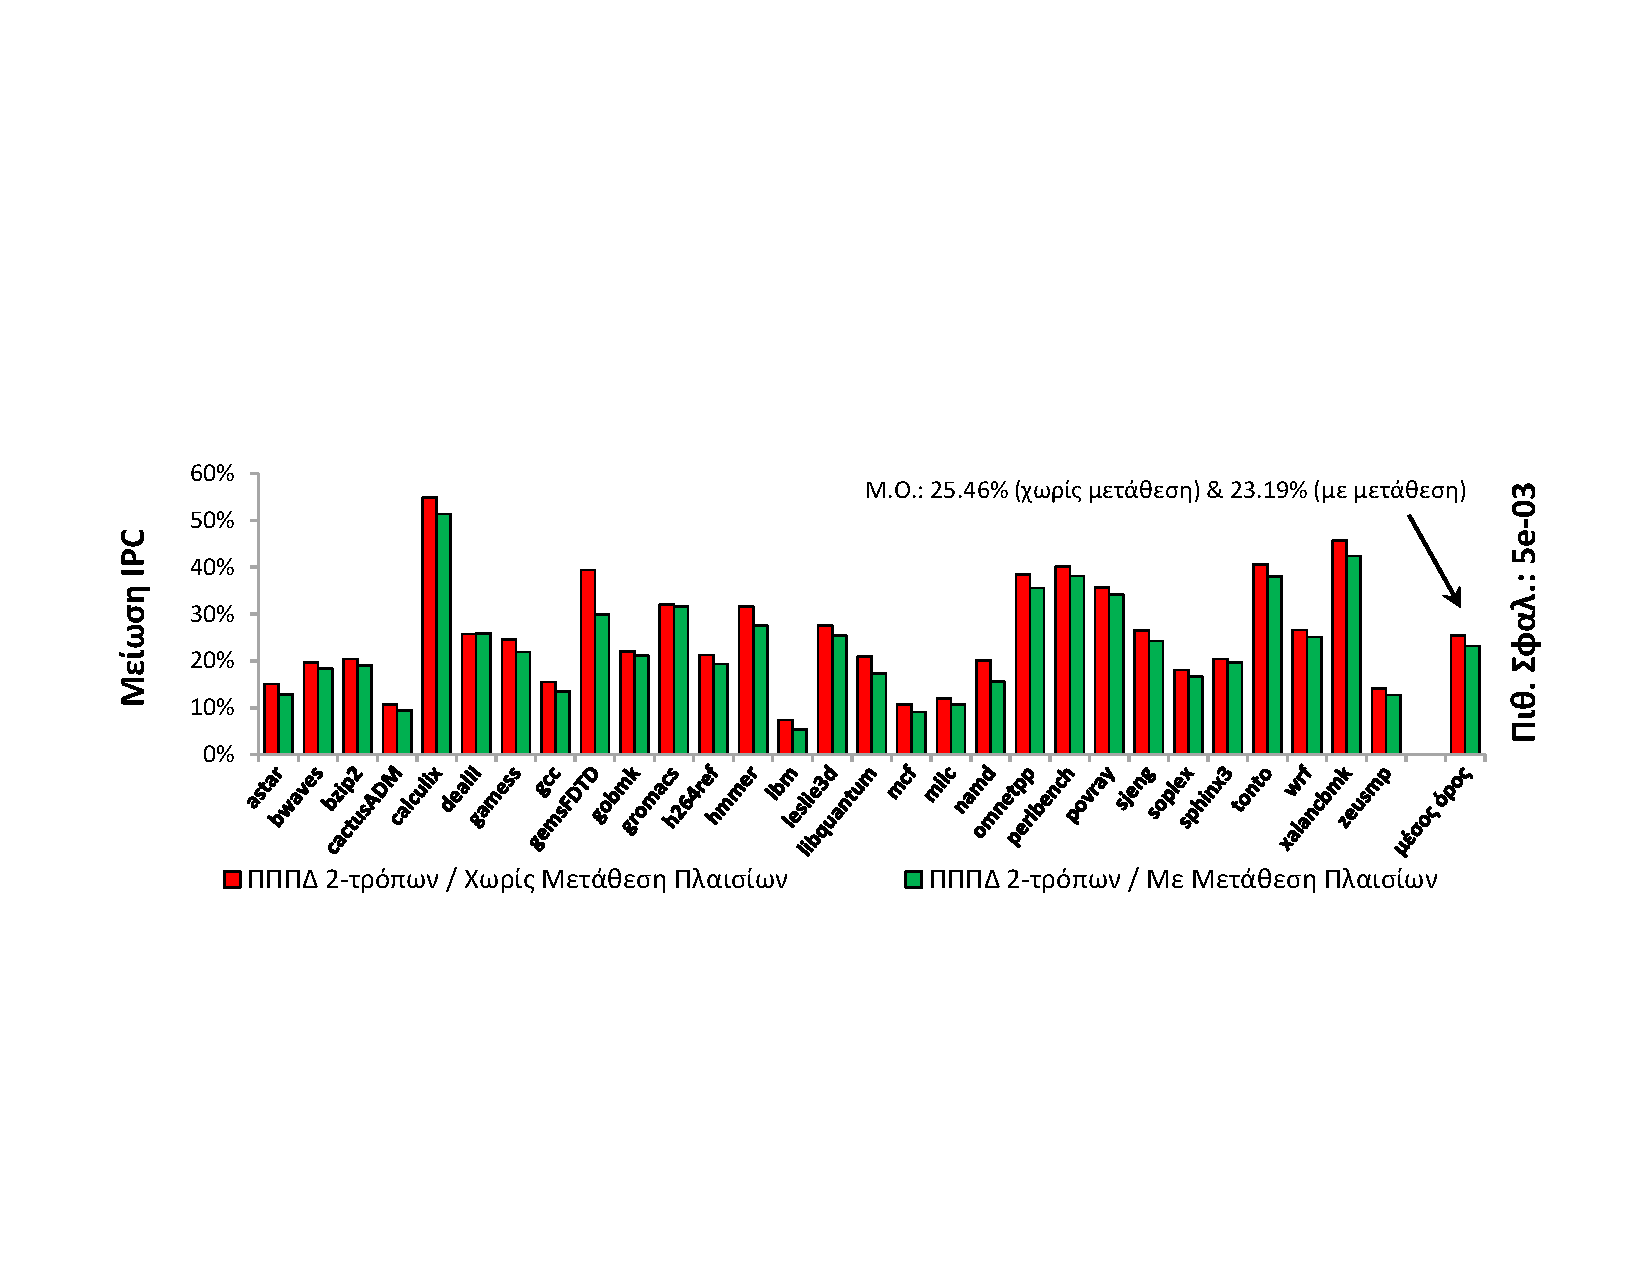
\includegraphics[width=\linewidth, trim=2cm 6.4cm 1.6cm 7.8cm, clip=true]{\resultsDIR/chap6_BTB_ipc_serial_w2_pfail2.pdf}}
        \caption{Πιθανότητα Σφάλματος 2}
        \label{fig:chap6_serial_2way_pail2_ipc}
    \end{subfigure}
    
    \caption{Αποτελέσματα με χρήση του σειριακού αλγορίθμου - (2-τρόπων ΠΠΠΔ)}
    \label{fig:chap6_serial_2way_ipc}
\end{figure}

Σύμφωνα με το γράφημα \ref{fig:chap6_serial_2way_pail2_ipc}, στην περίπτωση της πιθανότητας σφάλματος $\expnum{5}$, όπου τα ελαττωματικά πλαίσια ξεπερνούν το $40\%$, η μείωση του \ipc μεταβάλλεται κατά μέσο όρο από $25.5\%$ σε $23.2\%$ (επαναφορά κατά $8.9\%$). Η αδυναμία προσφοράς μεγαλύτερης επαναφοράς οφείλεται στον περιορισμό αναδιάταξης ενός μεγάλου πλήθους ελαττωματικών πλαισίων με αποδοτικό τρόπο όταν ο αριθμός τμημάτων είναι μικρός και χρησιμοποιείται ένας καταχωρητής ανά τμήμα (Σχήμα \ref{fig:chap5_btb_ffsets_2048_2way}: μείωση πλήρως ελαττωματικών συνόλων κατά 13\%). Παρόλα αυτά, υπάρχουν ορισμένες περιπτώσεις μετροπρογραμμάτων όπου η επαναφορά της απόδοσης είναι αρκετά σημαντική, όπως για παράδειγμα το \en{gemsFDTD} όπου η μείωση του \ipc μεταβάλλεται από $39.4\%$ σε $30\%$ (επαναφορά κατά $24\%$).
\par
Αντιστοίχως, το Σχήμα \ref{fig:chap6_serial_4way_ipc} αποτελείται από τις γραφικές παραστάσεις των περιπτώσεων Πινάκων Πρόβλεψης Προορισμού Διακλάδωσης 4-τρόπων. Το γράφημα \ref{fig:chap6_serial_4way_pail1_ipc} αναφέρεται στην περίπτωση της πιθανότητας σφάλματος $\expnum{2}$. H μείωση του \ipc ελαττώνεται κατά μέσο όρο από $1.20\%$ σε $0.63$\% ($47\%$ επαναφορά). Το σχετικά μικρό πλήθος ελαττωματικών συνόλων στην περίπτωση αυτή (λιγότερα από $20\%$) συνεπάγεται και την ελαχιστοποίηση της πιθανότητας να συνυπάρξουν 4 ελαττωματικά πλαίσια στο ίδιο σύνολο εξ αρχής. Για το λόγο αυτό η αρχική πτώση της απόδοσης δεν θεωρείται σημαντική, πλην ορισμένων περιπτώσεων όπως για παράδειγμα το \en{xalanbmk} όπου η μείωση της απόδοσης μεταβάλλεται από $8.5\%$ σε $6.5\%$ (επαναφορά κατά $23.7\%$).
\par
Στην πιθανότητα σφάλματος $\expnum{5}$, τα αποτελέσματα της οποίας παρουσιάζονται στο γράφημα \ref{fig:chap6_serial_4way_pail2_ipc}, η μείωση του \ipc ελαττώνεται κατά μέσο όρο από $8.1\%$ σε $3.8\%$. Συνεπώς η επαναφορά της απόδοσης είναι $52.9\%$. Παρότι το αρχικό ποσοστό μείωσης της απόδοσης δεν φαίνεται ιδιαίτερα σημαντικό, σε ορισμένα μετροπρογράμματα η βελτίωση είναι ιδιαίτερα σημαντική όπως για παράδειγμα το \en{calculix} όπου η μείωση της απόδοσης μεταβάλλεται από $19.6\%$ σε $7.6\%$ (επαναφορά κατά $61.2\%$).
\par
Στην περαιτέρω βελτίωση του ποσοστού επαναφοράς της απόδοσης σημαντικό ρόλο διαδραματίζει η χρήση περισσότερων Καταχωρητών Διαμόρφωσης ανά τμήμα, σύμφωνα με την μεθοδολογία που παρουσιάστηκε στην Ενότητα \ref{chap5_ImprovedMethod}.

\begin{figure}[!t]
    \centering
    \begin{subfigure}[t]{\textwidth}
        \centering
        \fbox{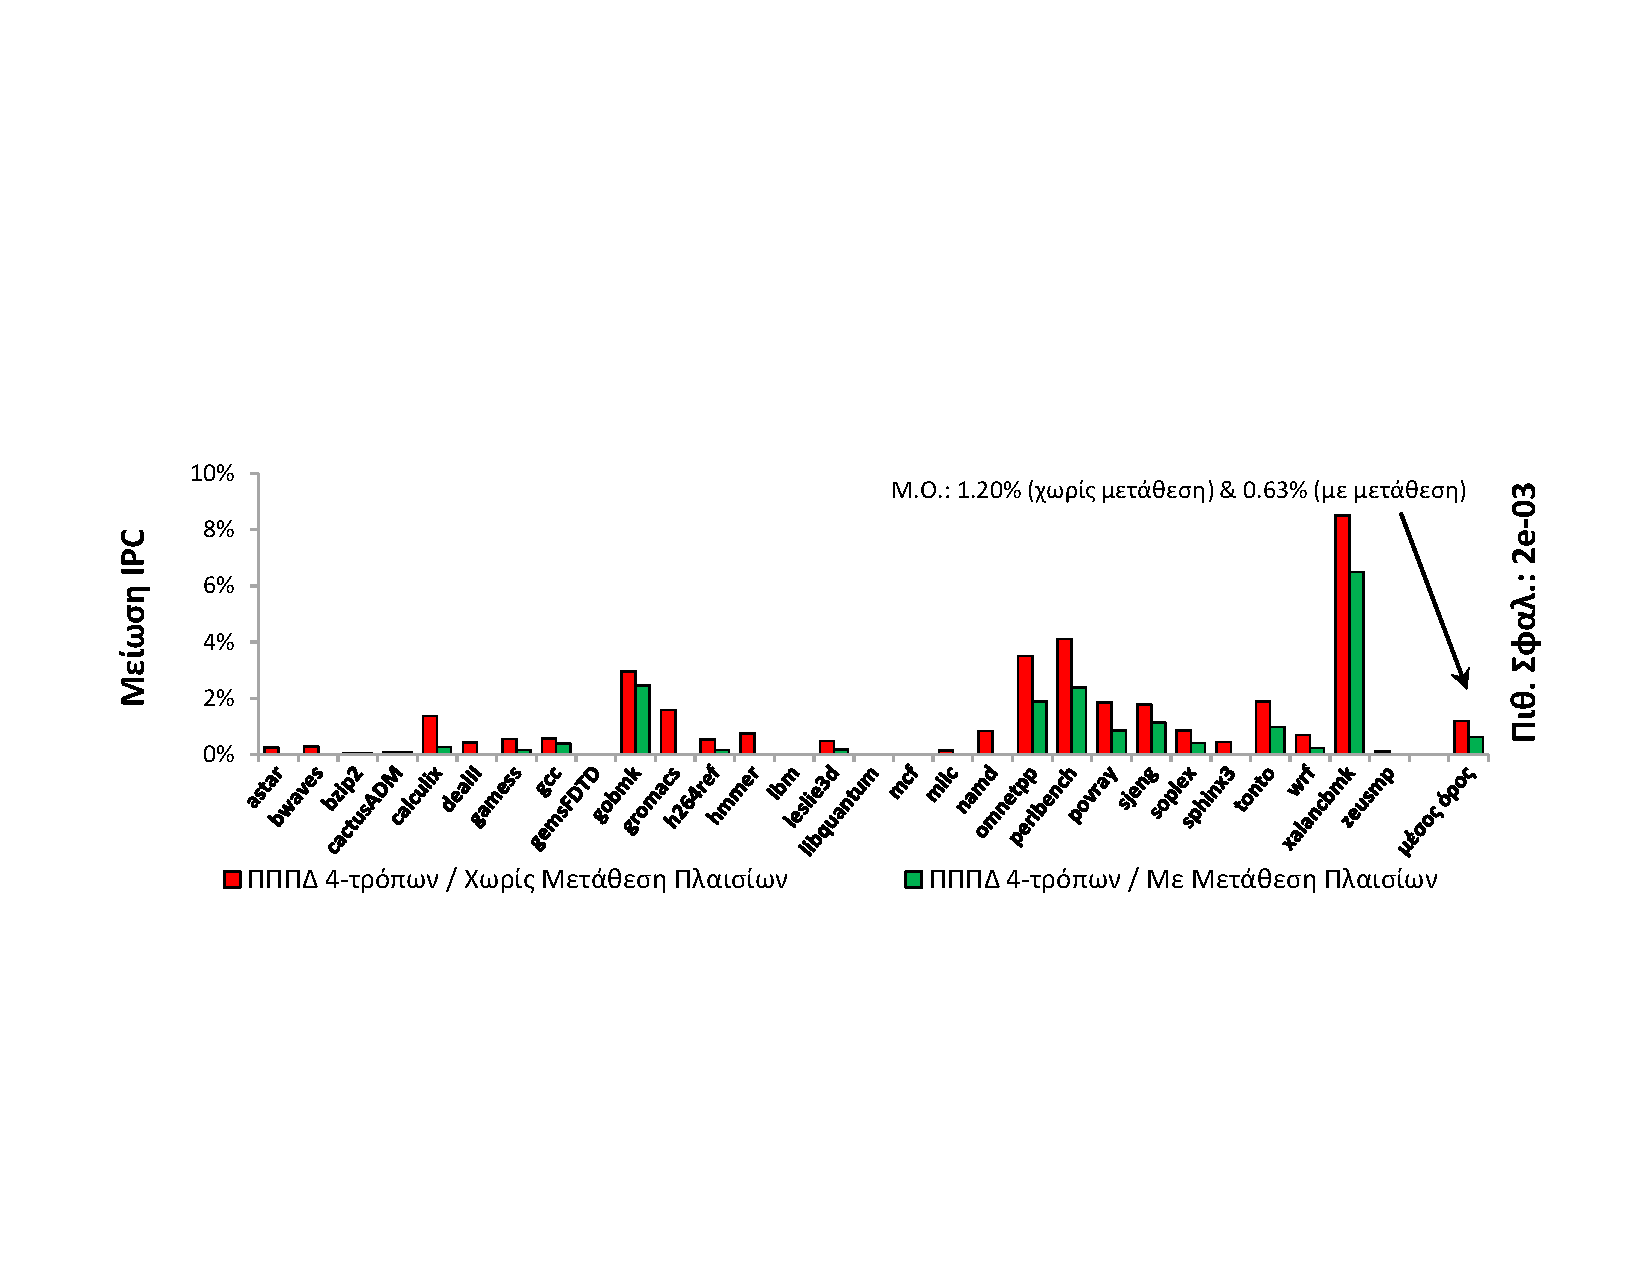
\includegraphics[width=\linewidth, trim=2cm 6.4cm 1.6cm 7.8cm, clip=true]{\resultsDIR/chap6_BTB_ipc_serial_w4_pfail1.pdf}}
        \caption{Πιθανότητα Σφάλματος 1}
        \label{fig:chap6_serial_4way_pail1_ipc}
    \end{subfigure}
    
    \begin{subfigure}[t]{\textwidth}
        \centering
        \fbox{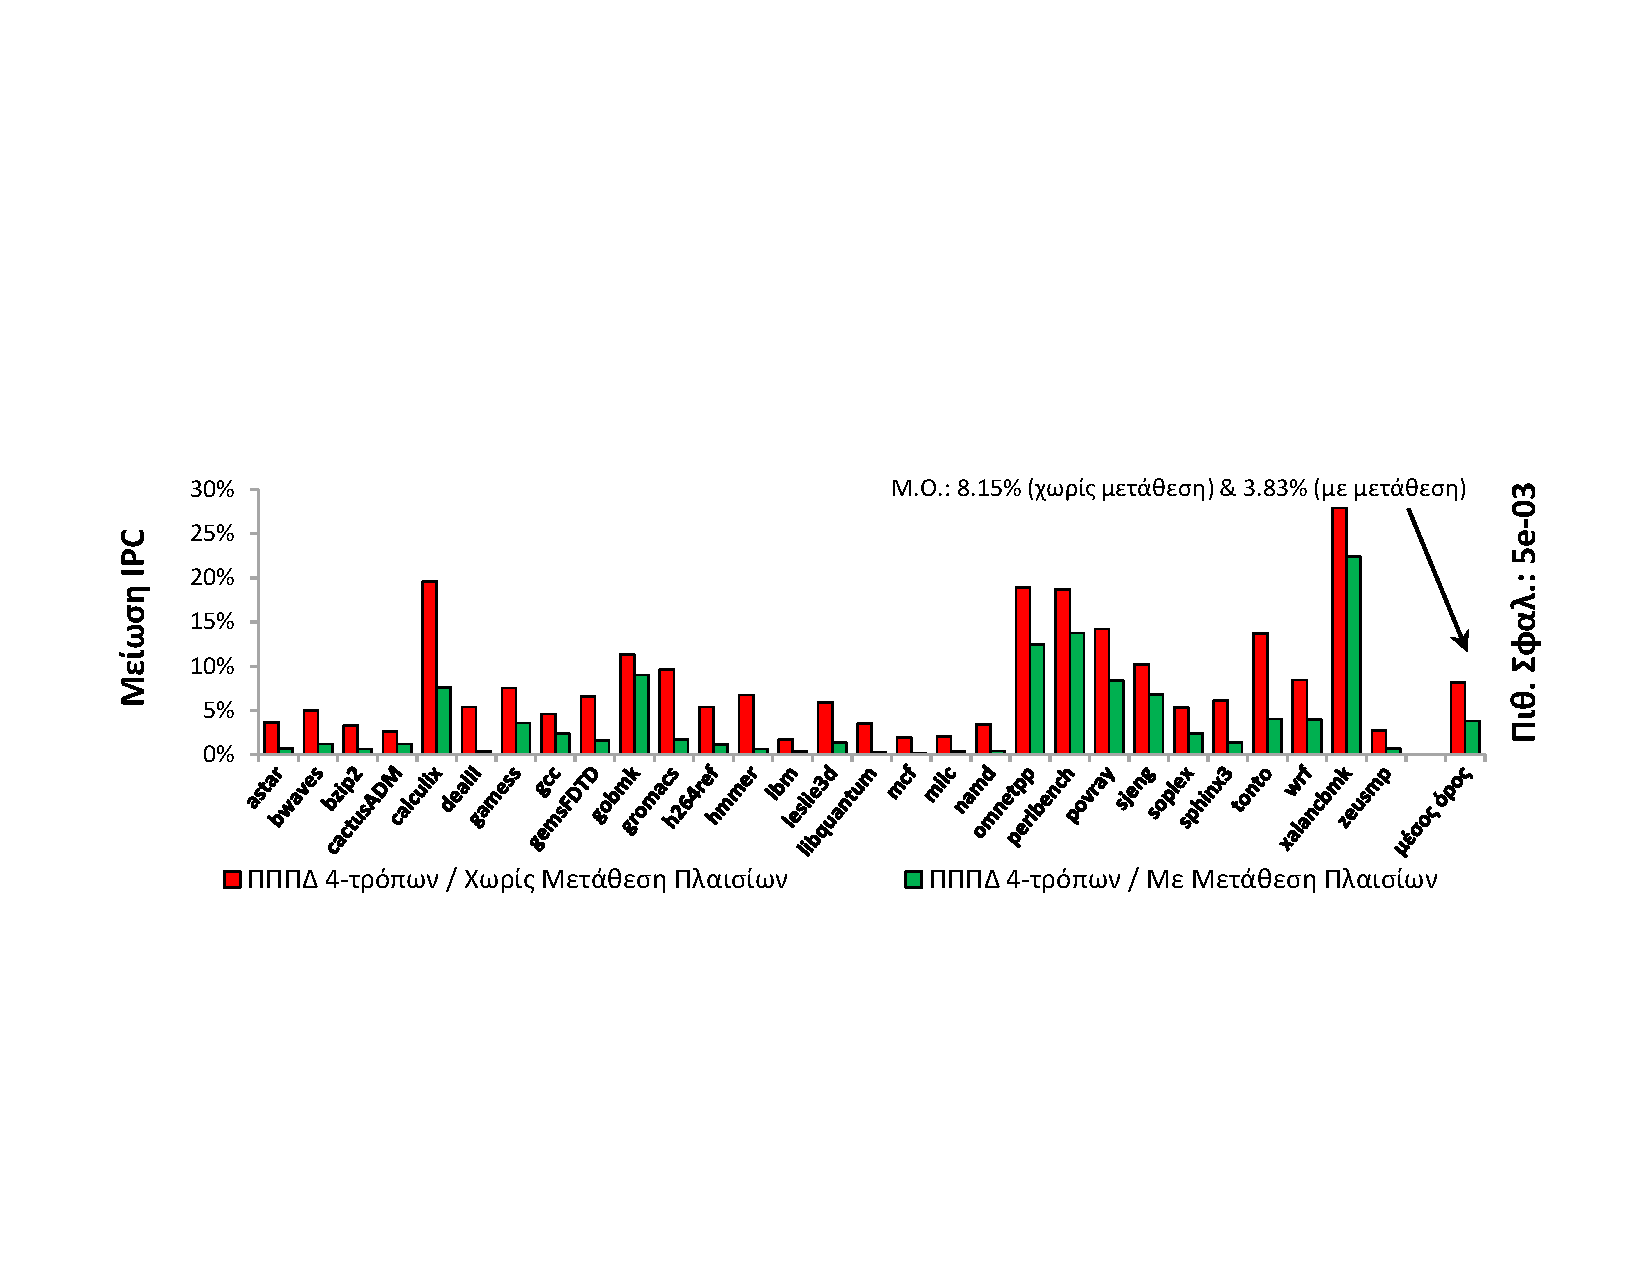
\includegraphics[width=\linewidth, trim=2cm 6.4cm 1.6cm 7.8cm, clip=true]{\resultsDIR/chap6_BTB_ipc_serial_w4_pfail2.pdf}}
        \caption{Πιθανότητα Σφάλματος 2}
        \label{fig:chap6_serial_4way_pail2_ipc}
    \end{subfigure}
    \caption{Αποτελέσματα με χρήση του σειριακού αλγορίθμου - (4-τρόπων ΠΠΠΔ)}
    \label{fig:chap6_serial_4way_ipc}
\end{figure}

%----------------------------------------------------------%

\subsection{Αποτελέσματα Ενισχυμένου Παράλληλου Μοντέλου}
\label{chap6_gem5ParallelAlgResults}

Στα γραφήματα του Σχήματος \ref{fig:chap6_parallel_4way_ipc} παρουσιάζεται η σύγκριση μεταξύ βασικού και ενισχυμένου μοντέλου όταν χρησιμοποιείται ο παράλληλος αλγόριθμος. Όπως αναφέρεται και στον Πίνακα \ref{tab:chap6_LowPowerSimulations}, πραγματοποιήθηκαν εξομοιώσεις για οργάνωση 4-τρόπων συνόλου συσχέτισης.
\par
Στην περίπτωση της πιθανότητας σφάλματος $\expnum{2}$ (γράφημα \ref{fig:chap6_parallel_4way_pail1_ipc}) η μείωση του \ipc εξαιτίας των σφαλμάτων στον Πίνακα Πρόβλεψης Προορισμού Διακλάδωσης ελαττώνεται κατά μέσο όρο από $1.20\%$ σε $0.73\%$. Επομένως, τεχνική της λογικής μετάθεσης πλαισίων ενός καταχωρητή ανά τμήμα, σε συνδυασμό με τη χρήση του παράλληλου αλγορίθμου μπορεί να επαναφέρει κατά $38.7\%$ την απόδοσης του υπερβαθμωτού επεξεργαστή, σε αντίθεση με την επαναφορά κατά $47\%$ που παρουσίασε η χρήση του σειριακού αλγορίθμου. Στην πιθανότητα σφάλματος $\expnum{5}$ (γράφημα \ref{fig:chap6_parallel_4way_pail2_ipc}) η μείωση του \ipc ελαττώνεται κατά μέσο όρο από $8.1\%$ σε $4.2\%$. Συνεπώς η επαναφορά της απόδοσης είναι $48\%$, από $52.9\%$ που ήταν με τη χρήση του σειριακού αλγορίθμου.
\par
Η διαφορά της βελτίωσης σε σχέση με την περίπτωση όπου χρησιμοποιείται ο σειριακός αλγόριθμος για τον υπολογισμό κατάλληλων τιμών ήταν αναμενόμενη σύμφωνα με την ανάλυση που πραγματοποιήθηκε στην Ενότητα \ref{chap5_AlgorithmResults}.

\begin{figure}[!t]
    \centering
    \begin{subfigure}[t]{\textwidth}
        \centering
        \fbox{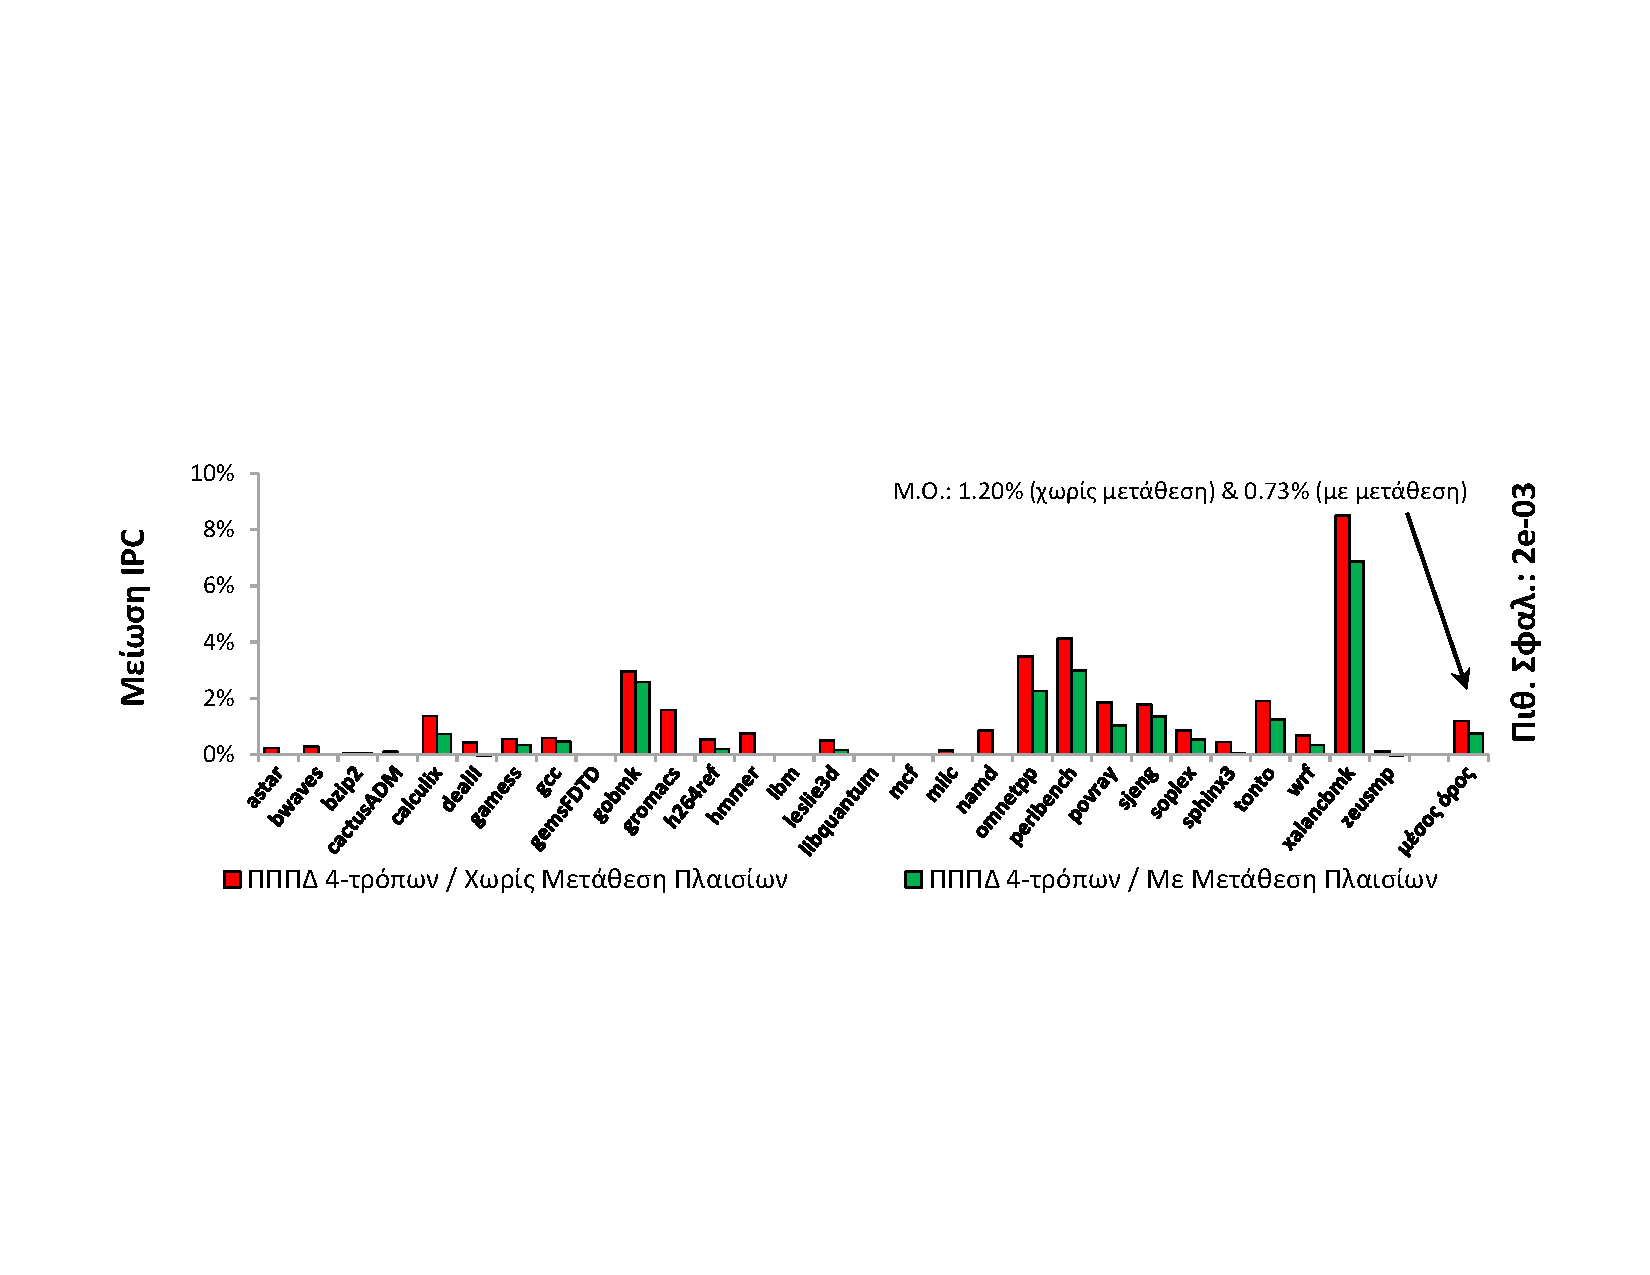
\includegraphics[width=\linewidth, trim=2cm 6.4cm 1.6cm 7.8cm, clip=true]{\resultsDIR/chap6_BTB_ipc_parallel_w4_pfail1.pdf}}
        \caption{Πιθανότητα Σφάλματος 1}
        \label{fig:chap6_parallel_4way_pail1_ipc}
    \end{subfigure}
    
    \begin{subfigure}[t]{\textwidth}
        \centering
        \fbox{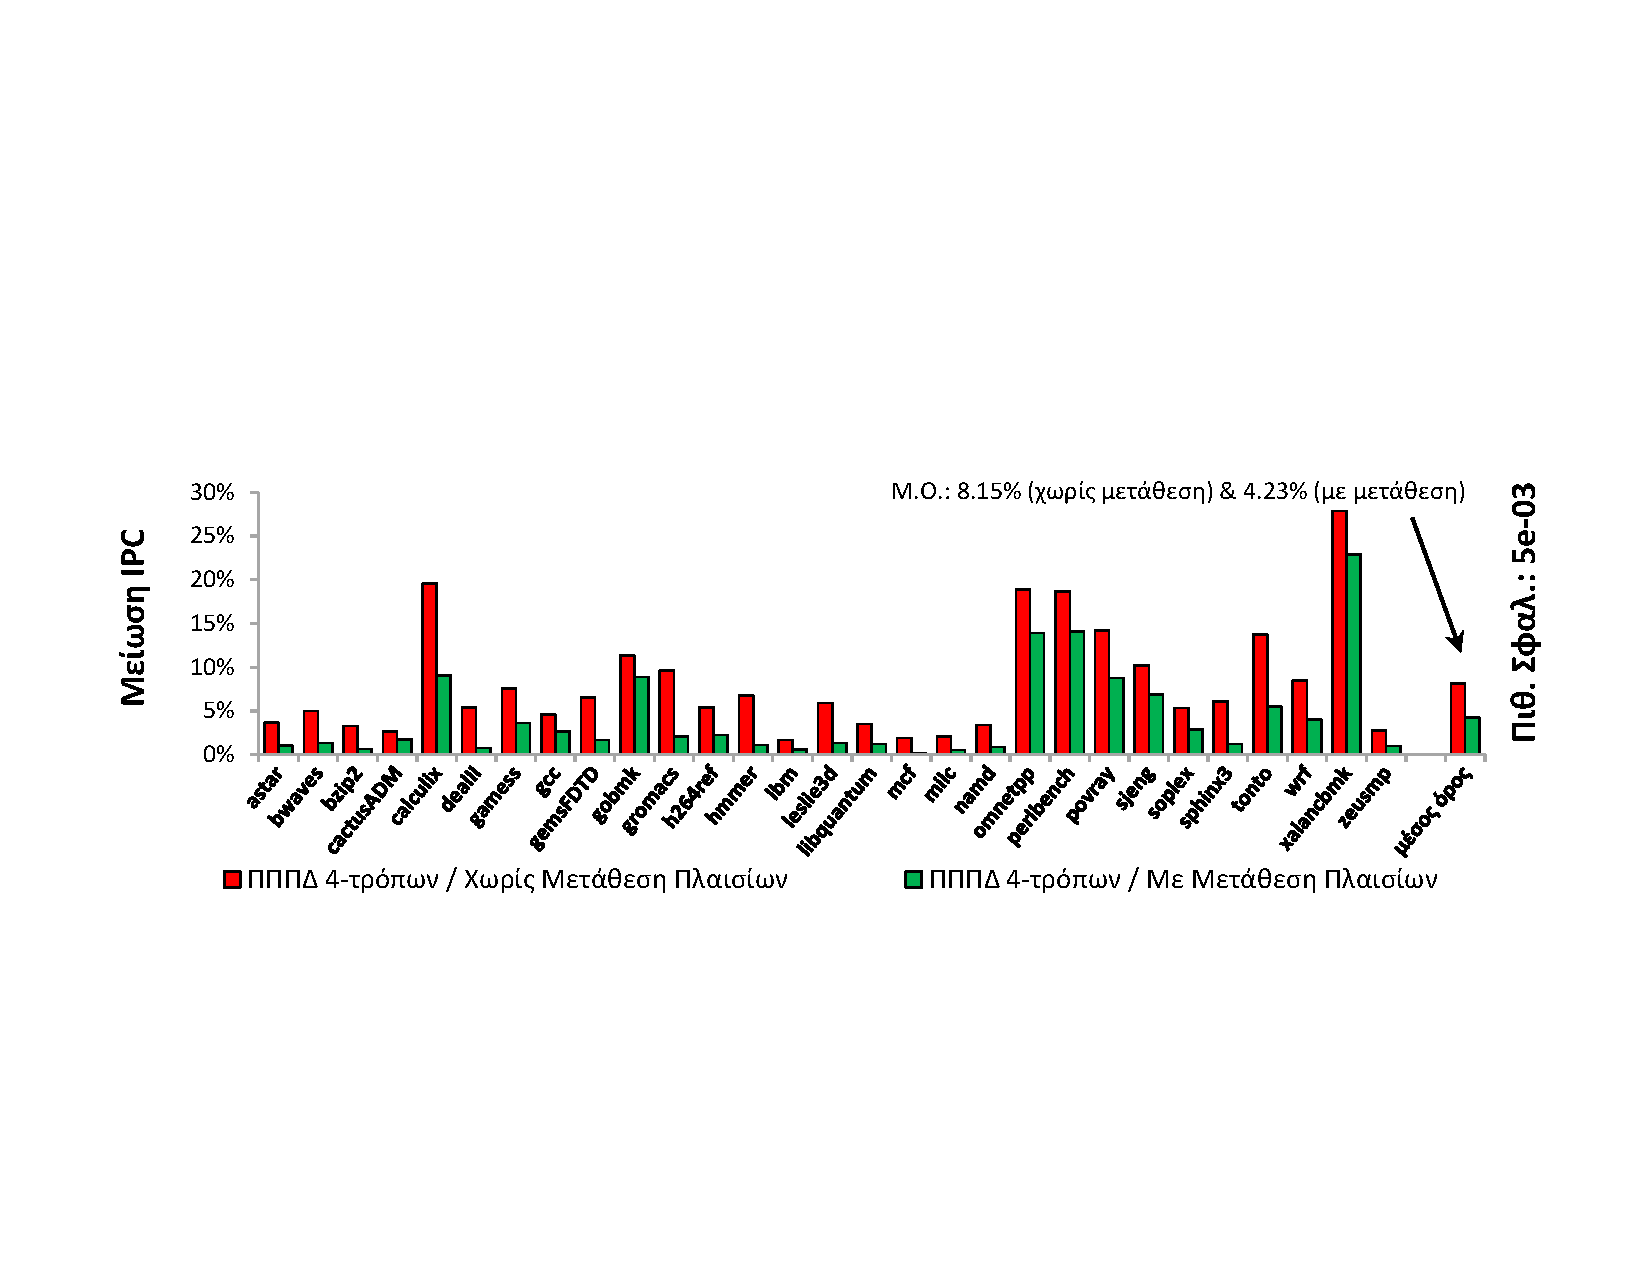
\includegraphics[width=\linewidth, trim=2cm 6.4cm 1.6cm 7.8cm, clip=true]{\resultsDIR/chap6_BTB_ipc_parallel_w4_pfail2.pdf}}
        \caption{Πιθανότητα Σφάλματος 2}
        \label{fig:chap6_parallel_4way_pail2_ipc}
    \end{subfigure}
    \caption{Αποτελέσματα με χρήση του παράλληλου αλγορίθμου}
    \label{fig:chap6_parallel_4way_ipc}
\end{figure}

%----------------------------------------------------------%

\subsection{Αποτελέσματα Βελτιστοποιημένου Σειριακού Μοντέλου}
\label{chap6_gem5OptimizedSerialAlgResults}

Η διάσπαση των τμημάτων σε υποτμήματα με τη χρήση ξεχωριστού Καταχωρητή Διαμόρφωσης σε κάθε ένα συμβάλει σημαντικά στην επίλυση του προβλήματος των πλήρως ελαττωματικών συνόλων. Τα αποτελέσματα της βελτιωμένης αυτής τεχνικής, παρουσιάζονται στα Σχήματα \ref{fig:chap6_optimized_serial_2way_ipc} και \ref{fig:chap6_optimized_serial_4way_ipc}, για οργανώσεις 2 και 4-τρόπων συνόλου συσχέτισης αντίστοιχα.
\par
Τα γραφήματα του Σχήματος \ref{fig:chap6_optimized_serial_2way_ipc} αναφέρονται στην περίπτωση οργάνωσης 2-τρόπων όπου κάθε τμήμα διασπάτε σε 64 υποτμήματα και επομένως κάθε Καταχωρητής Διαμόρφωσης συμβάλει στη δημιουργία 16 λογικών συνόλων. Στην πιθανότητα σφάλματος $\expnum{2}$, όπου η μείωση των πλήρως ελαττωματικών συνόλων αγγίζει το 95\% (Σχήμα \ref{fig:chap6_btb_ffsets_2048}), η μείωση του \ipc εξαιτίας των σφαλμάτων ελαττώνεται κατά μέσο όρο από $8.6\%$ σε $2.7\%$ (γράφημα \ref{fig:chap6_optimized_serial_2way_pail1_ipc}). Επομένως η επαναφορά της απόδοσης κατά μέσο όρο θα είναι $69\%$, από $32\%$ που ήταν με τη χρήση ενός μόνο καταχωρητή ανά τμήμα στην περίπτωση του ενισχυμένου σειριακού μοντέλου. Όπως φανερώνεται και από το γράφημα, σε ορισμένες περιπτώσεις μετροπρογραμμάτων επιτυγχάνεται πλήρης επαναφορά της απόδοσης όπως για παράδειγμα το \en{dealii} ($0\%$ μείωση του \ipc όταν εφαρμόζεται η τεχνική).
\par
Αντίστοιχα, στην περίπτωση της πιθανότητας σφάλματος $\expnum{5}$ (γράφημα \ref{fig:chap6_optimized_serial_2way_pail2_ipc}), όπου τα πλήρως ελαττωματικά σύνολα μειώνονται κατά 52\%, η μείωση του \ipc ελαττώνεται κατά μέσο όρο από $25.5\%$ σε $15.9\%$. Επομένως η επαναφορά της απόδοσης θα είναι $38\%$, από $9\%$ που ήταν με τη χρήση ενισχυμένου σειριακού μοντέλου. Σε αυτή την περίπτωση το μετροπρόγραμμα \en{gemsFDTD} εμφανίζει τη μεγαλύτερη βελτίωση καθώς η μείωση της απόδοσης μεταβάλλεται από $39.4\%$ σε $17.3\%$ (επαναφορά κατά $56\%$).

\begin{figure}[!t]
    \centering
    \begin{subfigure}[t]{\textwidth}
        \centering
        \fbox{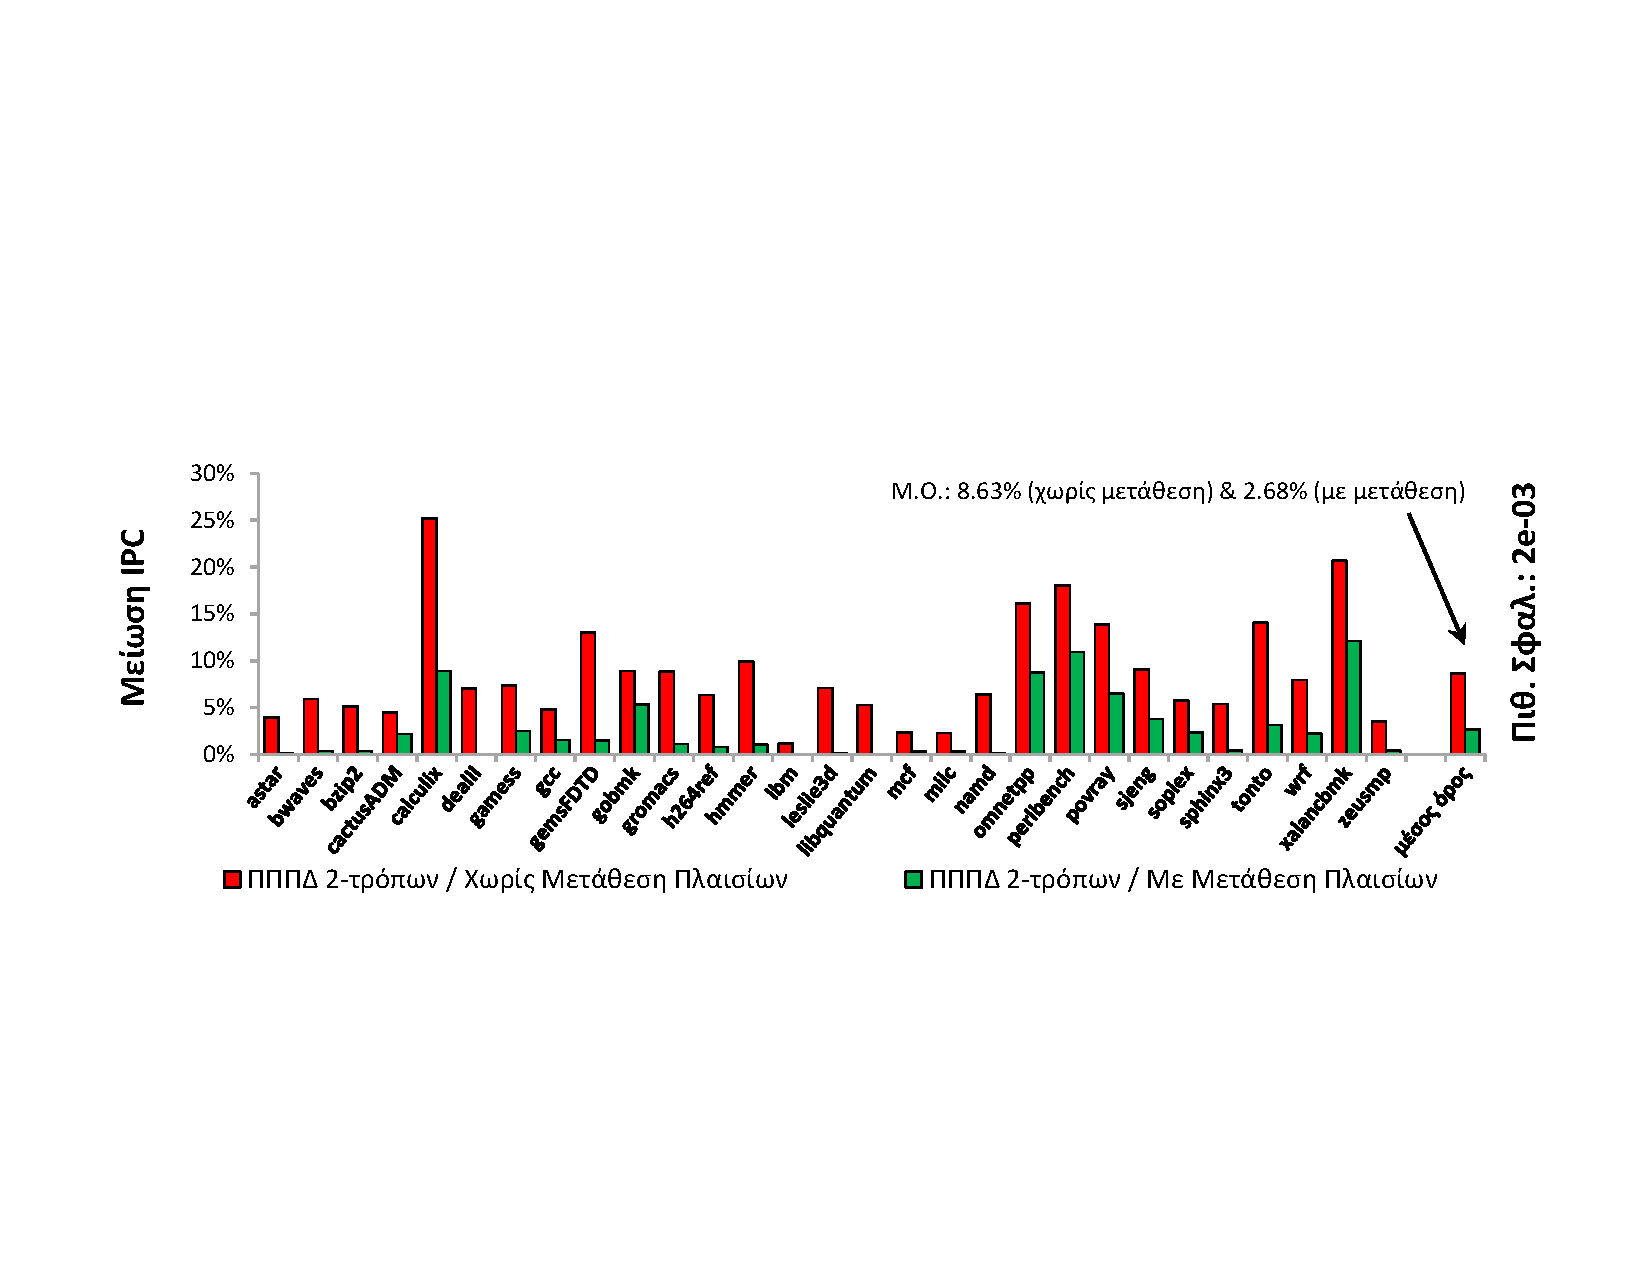
\includegraphics[width=\linewidth, trim=2cm 6.4cm 1.6cm 7.8cm, clip=true]{\resultsDIR/chap6_BTB_ipc_optimized_serial_w2_pfail1.pdf}}
        \caption{Πιθανότητα Σφάλματος 1}
        \label{fig:chap6_optimized_serial_2way_pail1_ipc}
    \end{subfigure}
    
    \begin{subfigure}[t]{\textwidth}
        \centering
        \fbox{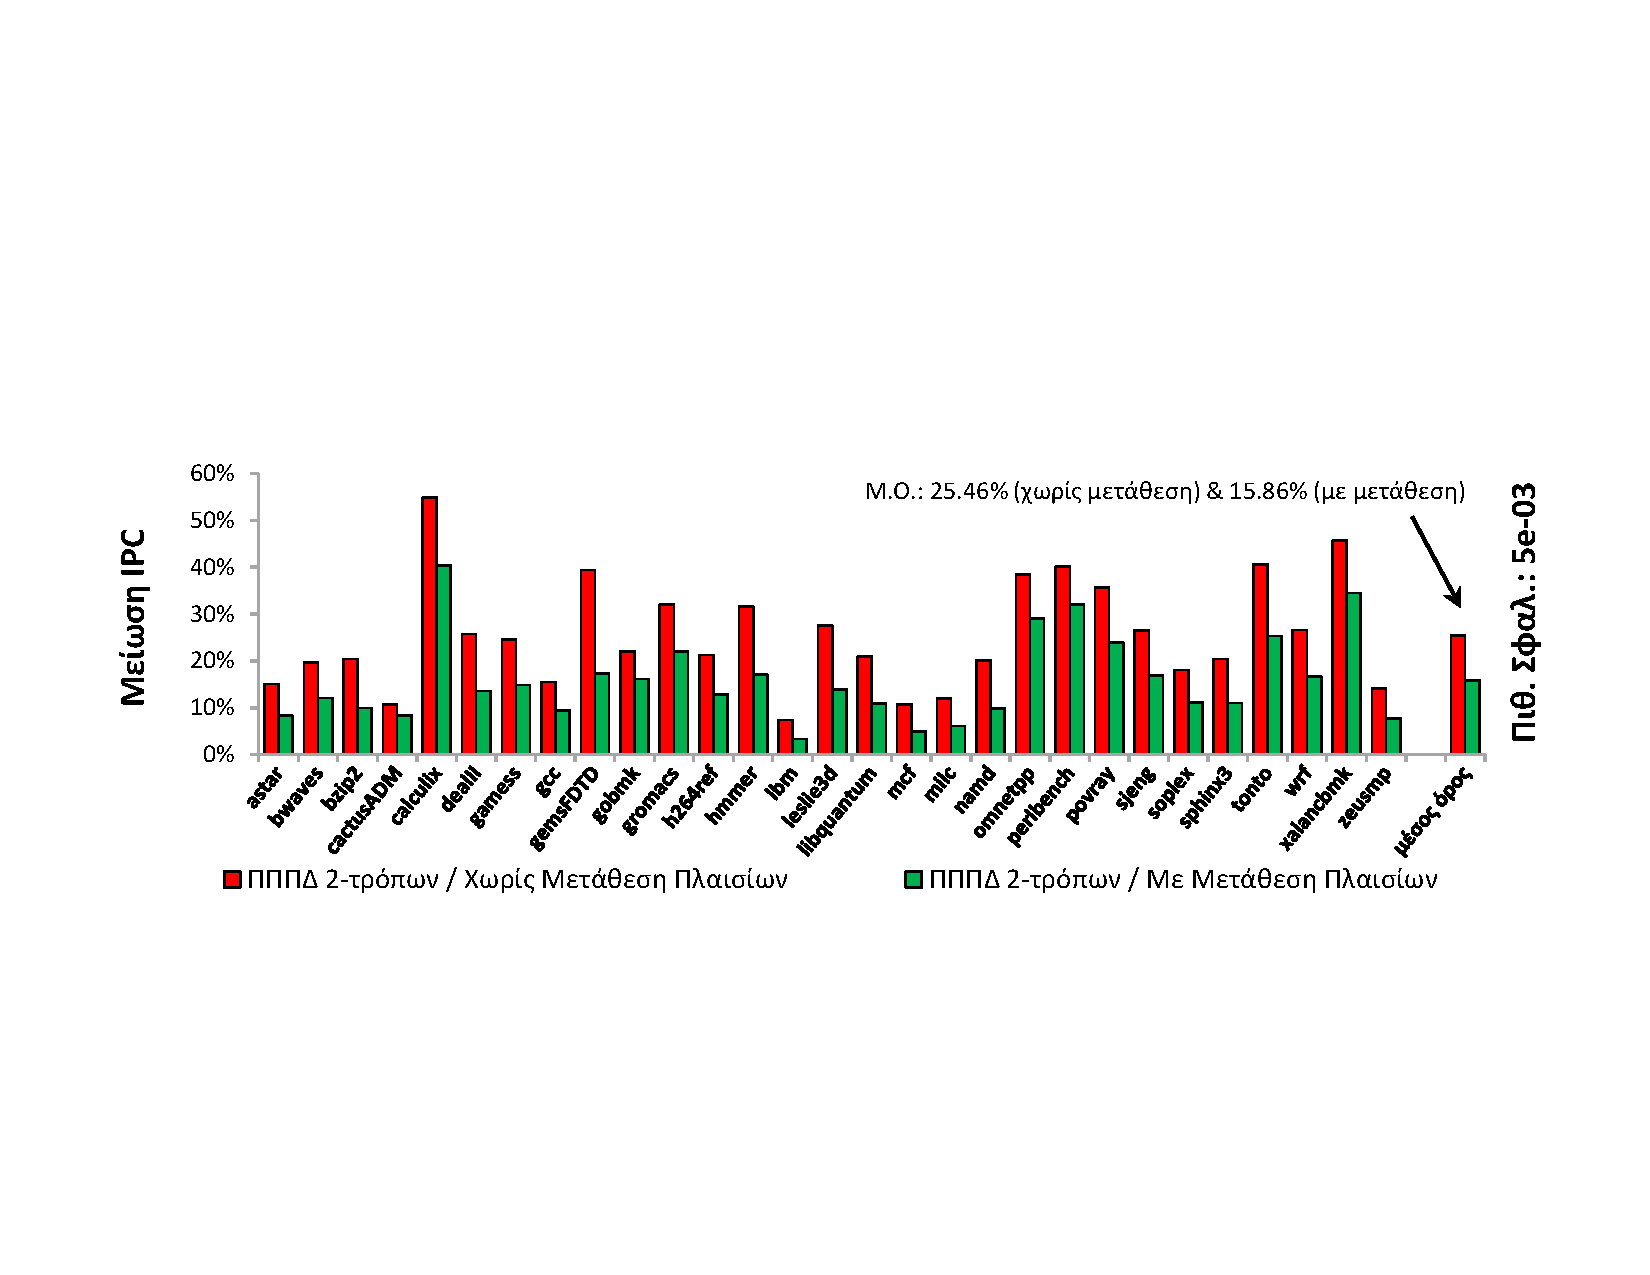
\includegraphics[width=\linewidth, trim=2cm 6.4cm 1.6cm 7.8cm, clip=true]{\resultsDIR/chap6_BTB_ipc_optimized_serial_w2_pfail2.pdf}}
        \caption{Πιθανότητα Σφάλματος 2}
        \label{fig:chap6_optimized_serial_2way_pail2_ipc}
    \end{subfigure}
    
    \caption{Αποτελέσματα με διάσπαση σε υποτμήματα και χρήση του σειριακού αλγορίθμου (2-τρόπων ΠΠΠΔ)}
    \label{fig:chap6_optimized_serial_2way_ipc}
\end{figure}

Το Σχήμα \ref{fig:chap6_optimized_serial_4way_ipc} αποτελείται από τις αντίστοιχες γραφικές παραστάσεις των περιπτώσεων Πινάκων Πρόβλεψης Προορισμού Διακλάδωσης 4-τρόπων. Τα αποτελέσματα της πιθανότητας σφάλματος $\expnum{2}$ παραλείπονται καθώς η χρήση τεσσάρων καταχωρητών ανά τμήμα κατά μέσο όρο προσφέρει ισοδύναμη επαναφορά της απόδοσης με την περίπτωση χρήση ενός καταχωρητή ανά τμήμα που παρουσιάστηκε στο ενισχυμένο σειριακό μοντέλο.
\par
Όταν η πιθανότητα σφάλματος είναι $\expnum{5}$ η χρήση μεγαλύτερου πλήθους καταχωρητών συμβάλει στην περαιτέρω βελτίωση τόσο της κατανομής όσο και της απόδοσης. Συγκεκριμένα, με τη χρήση 4 καταχωρητών ανά τμήμα, όπου εξασφαλίζεται η ολοκληρωτική εξάλειψη των πλήρως ελαττωματικών πλαισίων (Σχήμα \ref{fig:chap6_btb_ffsets_2048}), η μείωση του \ipc ελαττώνεται κατά μέσο όρο από $8.1\%$ σε $2.4\%$. Συνεπώς η επαναφορά της απόδοσης είναι $70\%$, από $52.9\%$ που ήταν με τη χρήση ενός καταχωρητή ανά τμήμα σε συνδυασμό με τη χρήση του σειριακού αλγορίθμου. Αξίζει να σημειωθεί πως και σε αυτή την περίπτωση πολλά μετροπρογράμματα αποκομίζουν σημαντικά οφέλη στην απόδοση, όπως για παράδειγμα το \en{calculix} όπου η μείωση της απόδοσης μεταβάλλεται από $19.6\%$ σε $3.3\%$ (επαναφορά κατά $83.1\%$).

\begin{figure}[!t]
    \centering
    \fbox{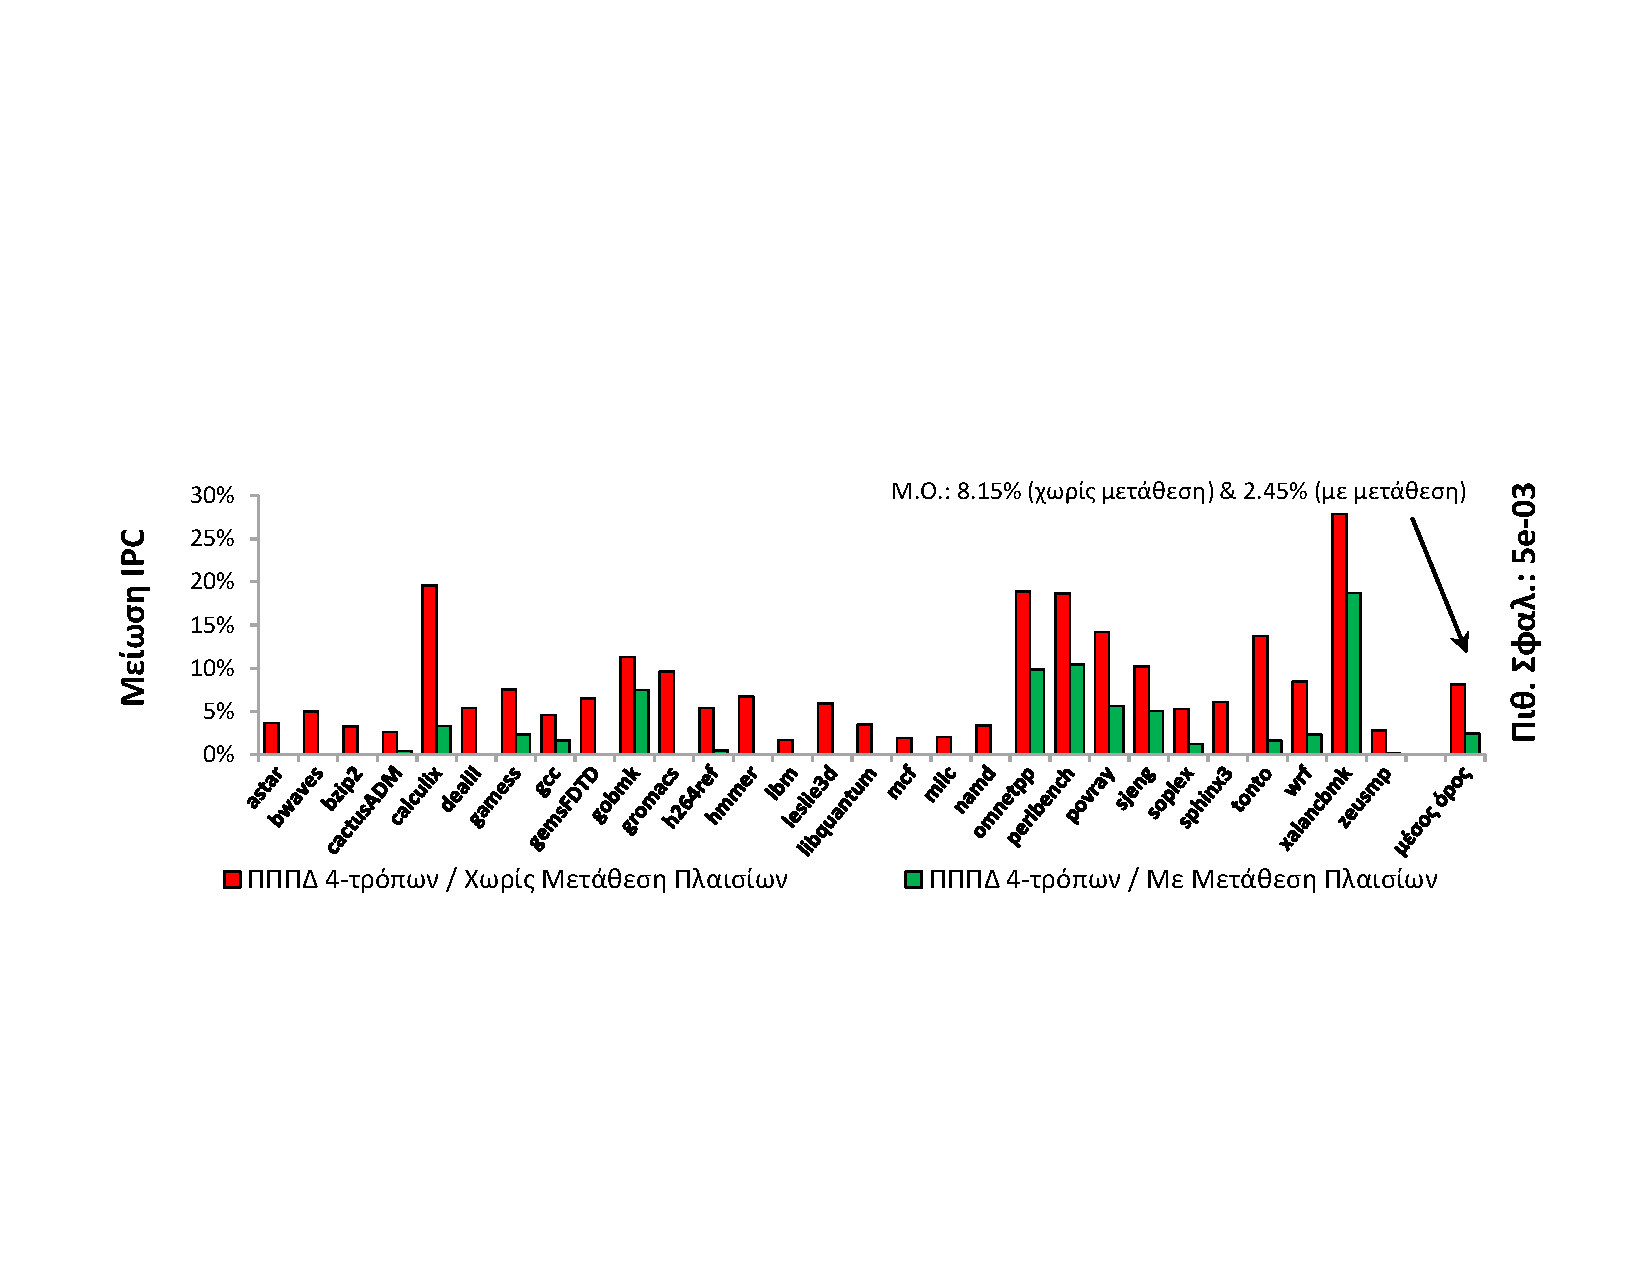
\includegraphics[width=\linewidth, trim=2cm 6.4cm 1.6cm 7.8cm, clip=true]{\resultsDIR/chap6_BTB_ipc_optimized_serial_w4_pfail2.pdf}}
    \caption{Αποτελέσματα με διάσπαση σε υποτμήματα και χρήση του σειριακού αλγορίθμου (4-τρόπων ΠΠΠΔ / Πιθανότητα Σφάλματος 2}
    \label{fig:chap6_optimized_serial_4way_ipc}
\end{figure}

%----------------------------------------------------------%

\section{Αποτελέσματα \mcpat}
\label{chap6_mcpatResults}

Σύμφωνα με τα αποτελέσματα της Ενότητας \ref{chap6_gem5Results}, η χρήση της προτεινόμενης μεθόδου με τις παραλλαγές που παρουσιάστηκαν εξασφαλίζει προστασία σε ικανοποιητικό επίπεδο ενάντια στην απώλεια απόδοσης, εξαιτίας της ύπαρξης σφαλμάτων στον Πίνακα Πρόβλεψης Προορισμού Διακλάδωσης. Το μέγεθος αυτής της βελτίωσης διαφέρει μεταξύ των μετροπρογραμμάτων και αυτό οφείλεται στη διαφορετική συμπεριφορά κάθε μετροπρογράμματος. Παρόλα αυτά, όταν ο υπερβαθμωτός επεξεργαστής λειτουργεί σε κατάσταση χαμηλής κατανάλωσης σημαντικότερη παράμετρο αξιολόγηση δεν αποτελεί η απόδοση σε επεξεργαστική ισχύ, αλλά η δυνατότητα μείωσης της συνολικής καταναλισκόμενης ενέργειας. Για το λόγο αυτό εκτελείται και η αντίστοιχη αξιολόγηση της προτεινόμενης μεθόδου, σε σχέση με το βασικό μοντέλο.
\par
Στην παρούσα αξιολόγηση υπολογίζεται η ενέργεια που δαπανάται για τη συνολική εκτέλεση ενός προγράμματος (Γινόμενο Ενέργειας-Καθυστέρησης - \edp) για κάθε εξομοιούμενο μοντέλο,
διότι η προτεινόμενη τεχνική δεν προσφέρει μείωση της κατανάλωσης ανά χρονική στιγμή αλλά μείωση του συνολικού χρόνου εκτέλεσης ενός προγράμματος, το οποίο συνεπάγεται τη μείωση της συνολικής κατανάλωσης.
\par
Στα ακόλουθα γραφήματα παρουσιάζεται η αύξηση της συνολικής κατανάλωσης που αντιστοιχεί στην αύξηση του \edp, το μέγεθος της οποίας υπολογίζεται από την εξίσωση:

\begin{equation}
    \label{eqn:chap6_EDPfaulty}
    \mathgr{Μείωση}\_EDP = \frac{EDP_\mathgr{χωρίς\_σφάλματα} - EDP_\mathgr{εξομοιούμενο\_μοντέλο\_με\_σφάλματα}}{EDP_\mathgr{χωρίς\_σφάλματα}}
\end{equation}

Σε αντίθεση με τα γραφήματα του \ipc που παρουσιάστηκαν έως τώρα, η αύξηση του \edp αποτελεί αρνητικό παράγοντα και επομένως ζητούμενο είναι η ελάττωση της. Το ποσοστό 0\% αντιστοιχεί σε μηδενική αύξηση της ενέργειας που πρόκειται να καταναλωθεί για την εκτέλεση του αντίστοιχου μετροπρογράμματος, εξαιτίας των σφαλμάτων (\edp με σφάλματα = \edp χωρίς σφάλματα). Όπως και στα γραφήματα της απόδοσης, η μεταβολή της κατανάλωσης παρουσιάζεται ξεχωριστά για κάθε μετροπρόγραμμα, με τις μπάρες πορτοκαλί αποχρώσεων να αντιστοιχούν στα αποτελέσματα του βασικού μοντέλου ενώ αυτές των μπλε αποχρώσεων στα αποτελέσματα του ενισχυμένου/βελτιστοποιημένου. Οι μελετώμενες πιθανότητες σφάλματος σε κάθε περίπτωση, όπως και στην περίπτωση της απόδοσης, είναι $\expnum{2}$ και $\expnum{5}$ (Πιθανότητα Σφάλματος 1 και Πιθανότητα Σφάλματος 2 αντίστοιχα).

%----------------------------------------------------------%

\subsection{Αποτελέσματα Ενισχυμένου Σειριακού Μοντέλου}
\label{chap6_mcpatSerialAlgResults}

Στα ακόλουθα Σχήματα \ref{fig:chap6_serial_2way_edp} και \ref{fig:chap6_serial_4way_edp} παρουσιάζεται η σύγκριση μεταξύ βασικού και ενισχυμένου μοντέλου όταν χρησιμοποιείται ο σειριακός αλγόριθμος για τις δύο οργανώσεις συνόλου συσχέτισης.
\par
Στην πιθανότητα σφάλματος $\expnum{2}$ και οργάνωση 2-τρόπων (γράφημα \ref{fig:chap6_serial_2way_pail1_edp}), η αύξηση του \edp ελαττώνεται κατά μέσο όρο από $28.76\%$ σε $16.85\%$. Επομένως η επαναφορά της κατανάλωσης είναι $41\%$. Μεταξύ των μετροπρογραμμάτων εμφανίζονται και περιπτώσεις όπου η επαναφορά είναι αρκετά μεγαλύτερη του μέσου όρου όπως για παράδειγμα το \en{gemsFDTD} όπου η αύξηση μεταβάλλεται από $120.74\%$ σε $44.56\%$ (επαναφορά κατά $63\%$).
\par
Αντίστοιχα, στο γράφημα \ref{fig:chap6_serial_2way_pail2_edp} παρουσιάζονται τα αποτελέσματα της πιθανότητας σφάλματος $\expnum{5}$ και οργάνωση 2-τρόπων. Η αύξηση του \edp σε αυτή την περίπτωση ελαττώνεται κατά μέσο όρο από $124.33\%$ σε $104.24\%$. Επομένως η επαναφορά της κατανάλωσης είναι $16\%$. Παρόλα αυτά, στο μετροπρόγραμμα \en{gemsFDTD} εμφανίζεται μεταβολή της αύξηση από $517.28\%$ σε $314.34\%$ (επαναφορά κατά $39\%$).

\begin{figure}[!t]
    \centering
    \begin{subfigure}[t]{\textwidth}
        \centering
        \fbox{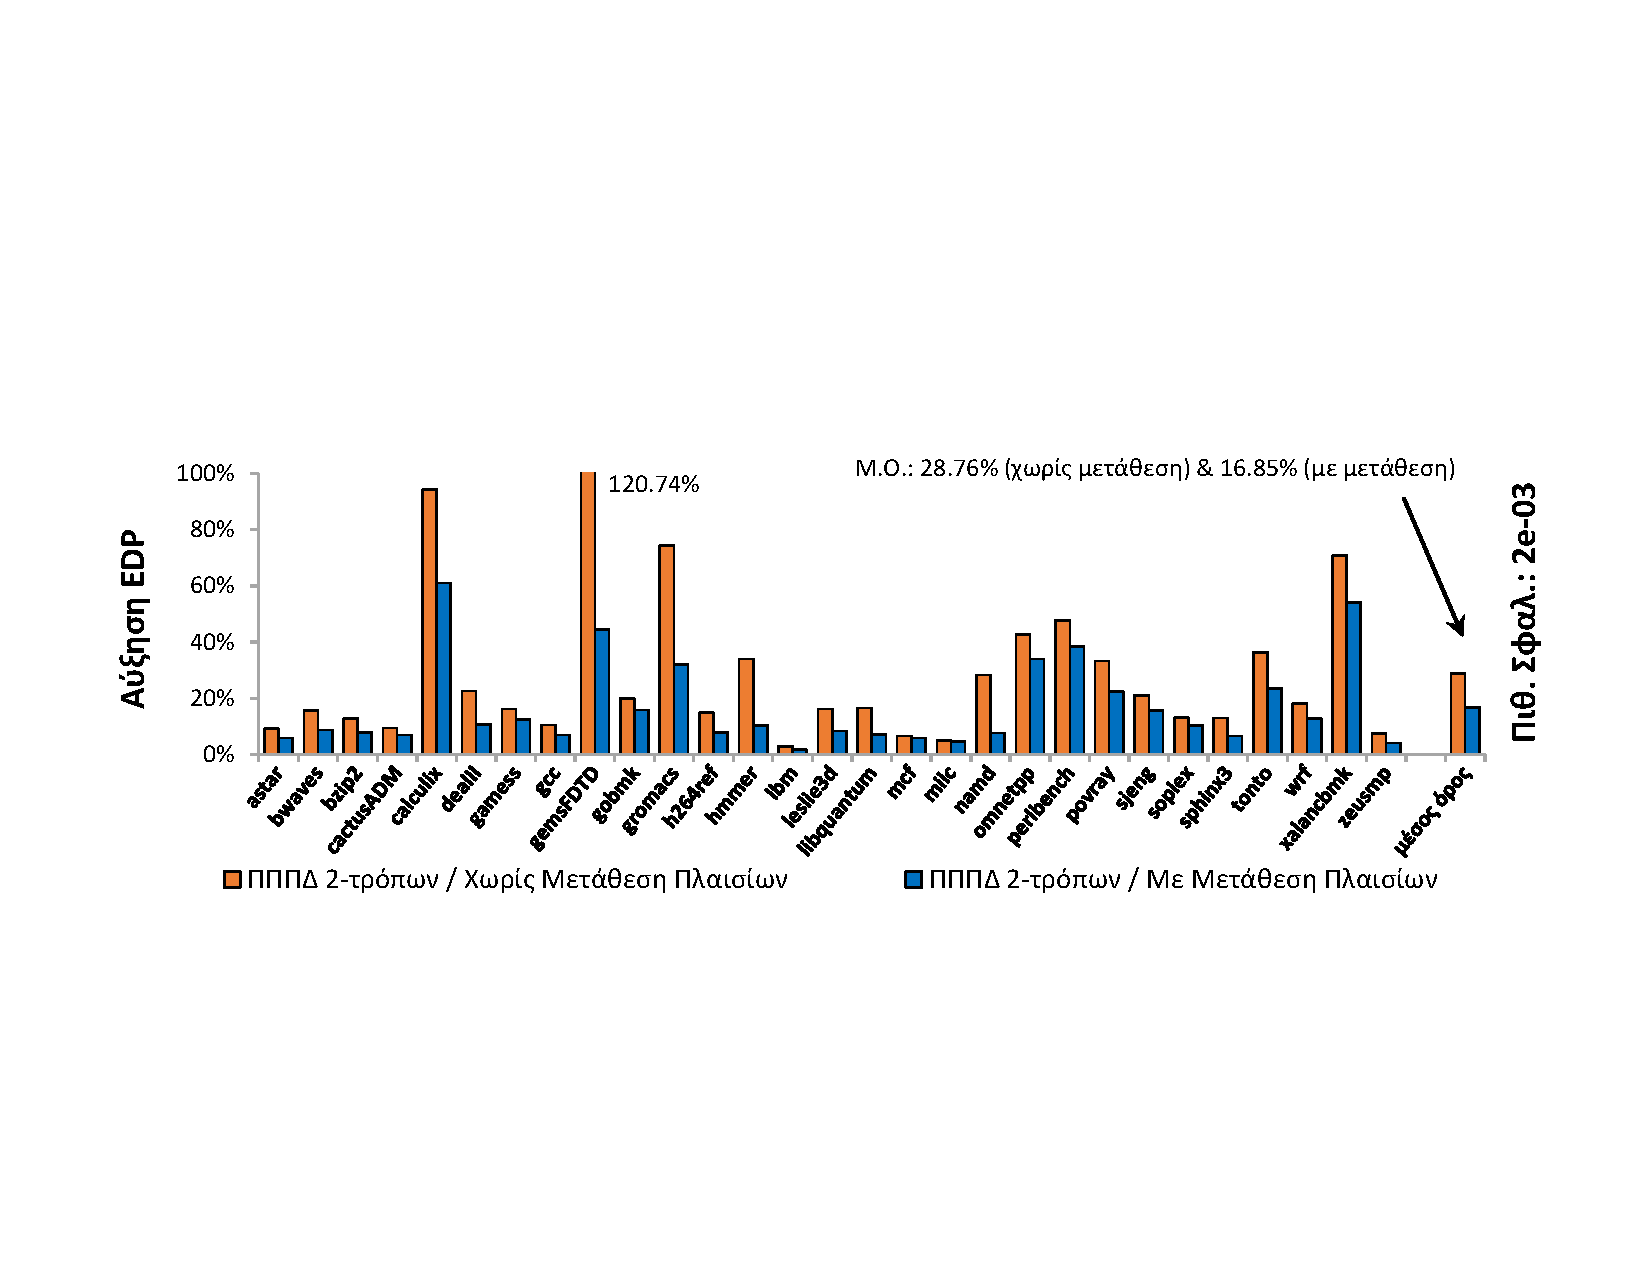
\includegraphics[width=\linewidth, trim=2cm 6.4cm 1.6cm 7.7cm, clip=true]{\resultsDIR/chap6_BTB_edp_serial_w2_pfail1.pdf}}
        \caption{Πιθανότητα Σφάλματος 1}
        \label{fig:chap6_serial_2way_pail1_edp}
    \end{subfigure}
    
    \begin{subfigure}[t]{\textwidth}
        \centering
        \fbox{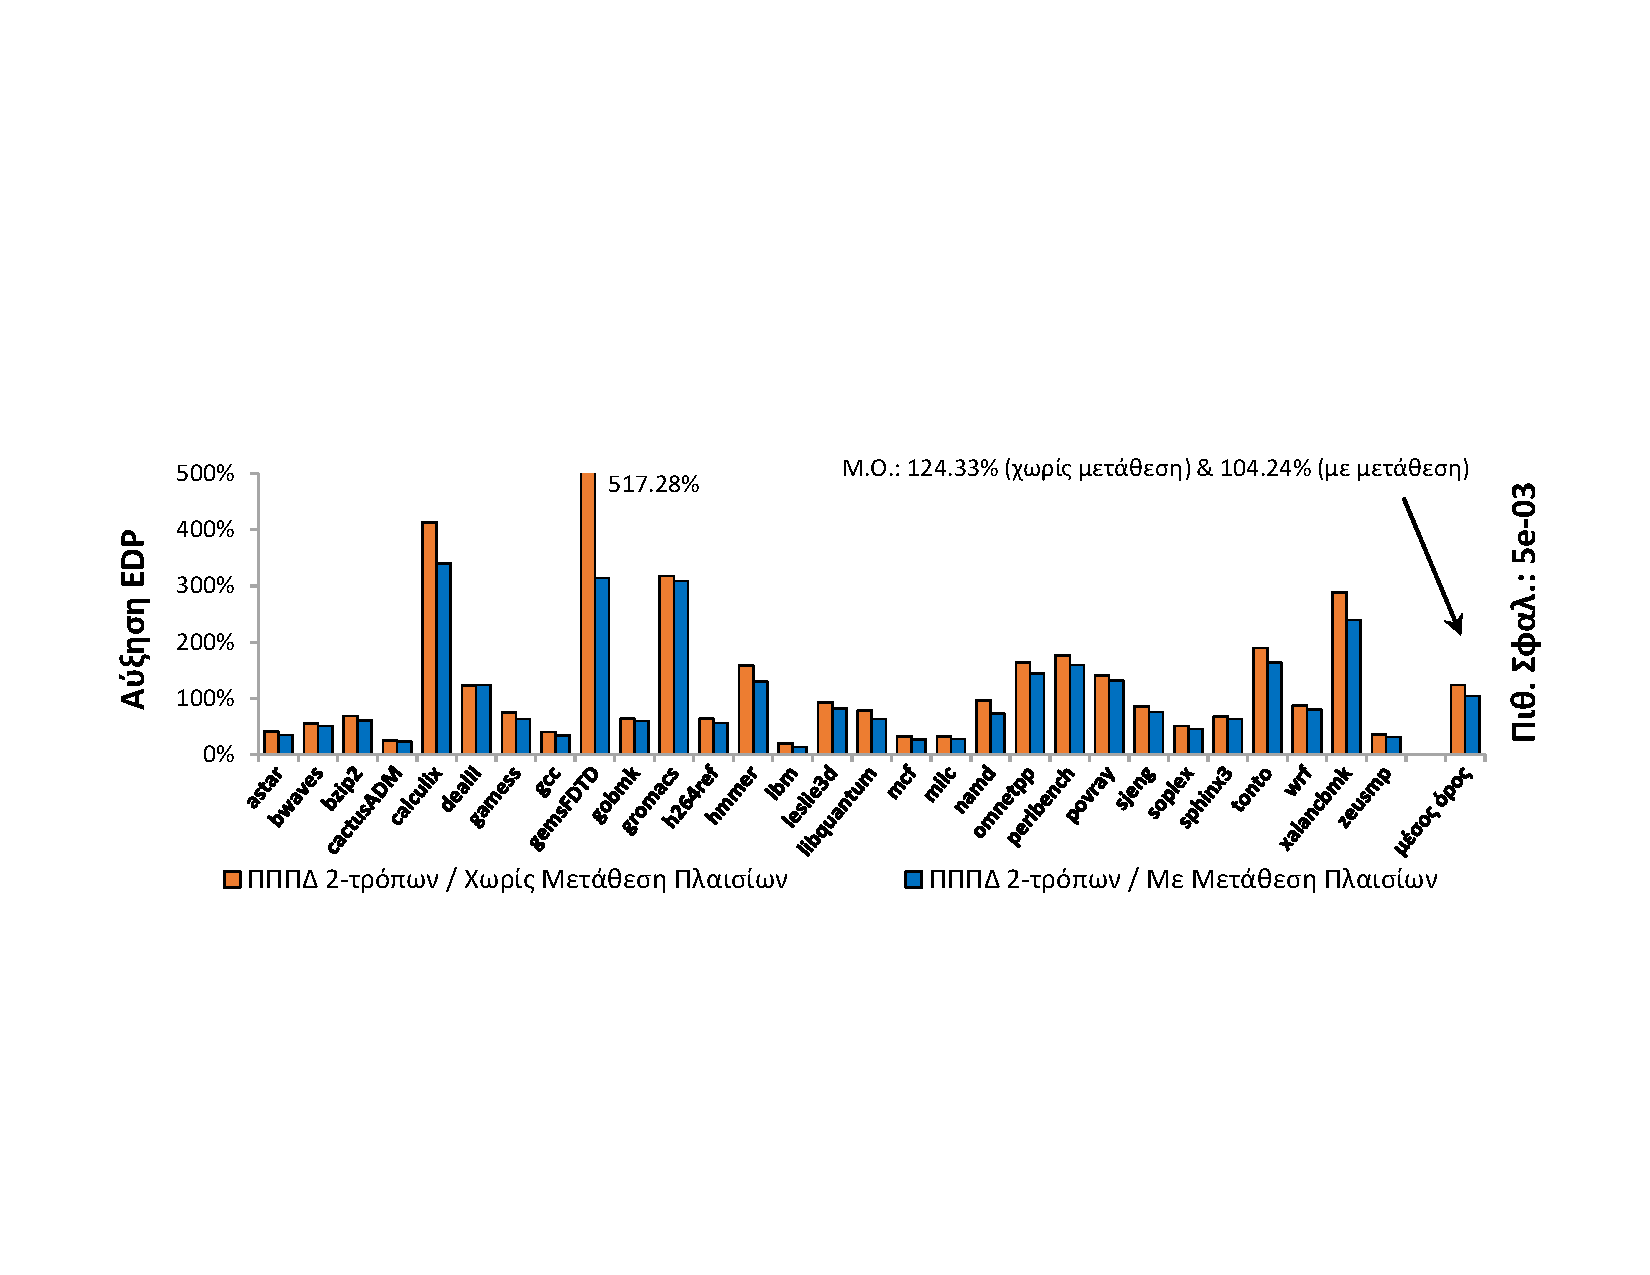
\includegraphics[width=\linewidth, trim=2cm 6.4cm 1.6cm 7.7cm, clip=true]{\resultsDIR/chap6_BTB_edp_serial_w2_pfail2.pdf}}
        \caption{Πιθανότητα Σφάλματος 2}
        \label{fig:chap6_serial_2way_pail2_edp}
    \end{subfigure}
    
    \caption{Αποτελέσματα με χρήση του σειριακού αλγορίθμου - (2-τρόπων ΠΠΠΔ)}
    \label{fig:chap6_serial_2way_edp}
\end{figure}

Όταν η οργάνωση είναι 4-τρόπων η ελάττωση των επιπτώσεων στην κατανάλωση εξαιτίας των σφαλμάτων στον Πίνακα Πρόβλεψης Προορισμού Διακλάδωσης γίνεται ευκολότερη. Στην πιθανότητα σφάλματος $\expnum{2}$ (γράφημα \ref{fig:chap6_serial_4way_pail1_edp}), η αύξηση του \edp ελαττώνεται κατά μέσο όρο από $2.93\%$ σε $1.34\%$ (επαναφορά κατά $54\%$). Στο μετροπρόγραμμα \en{gromacs} παρουσιάζεται η μεγαλύτερη βελτίωση καθώς η αύξηση της κατανάλωσης μεταβάλλεται από $11.92\%$ σε μόλις $0.11\%$ (επαναφορά κατά $99\%$). Συνεπώς η χρήση της προτεινόμενης τεχνικής έκανε το συγκεκριμένο μετροπρόγραμμα να εκτελεστεί με το ίδιο ενεργειακό κόστος που θα είχε εάν όλα τα πλαίσια του Πίνακα Πρόβλεψης Προορισμού Διακλάδωσης λειτουργούσαν σωστά.
\par
Στην πιθανότητα σφάλματος $\expnum{5}$ (γράφημα \ref{fig:chap6_serial_4way_pail2_edp}), η αύξηση του \edp ελαττώνεται κατά μέσο όρο από $25.92\%$ σε $9.87\%$ (επαναφορά κατά $62\%$). Όπως και στην χαμηλότερη πιθανότητα σφάλματος, το μετροπρόγραμμα \en{gromacs} παρουσιάζει τη μεγαλύτερη βελτίωση καθώς η αύξηση της κατανάλωσης μεταβάλλεται από $78.69\%$ σε $9.39\%$ (επαναφορά κατά $88\%$).

\begin{figure}[!t]
    \centering
    \begin{subfigure}[t]{\textwidth}
        \centering
        \fbox{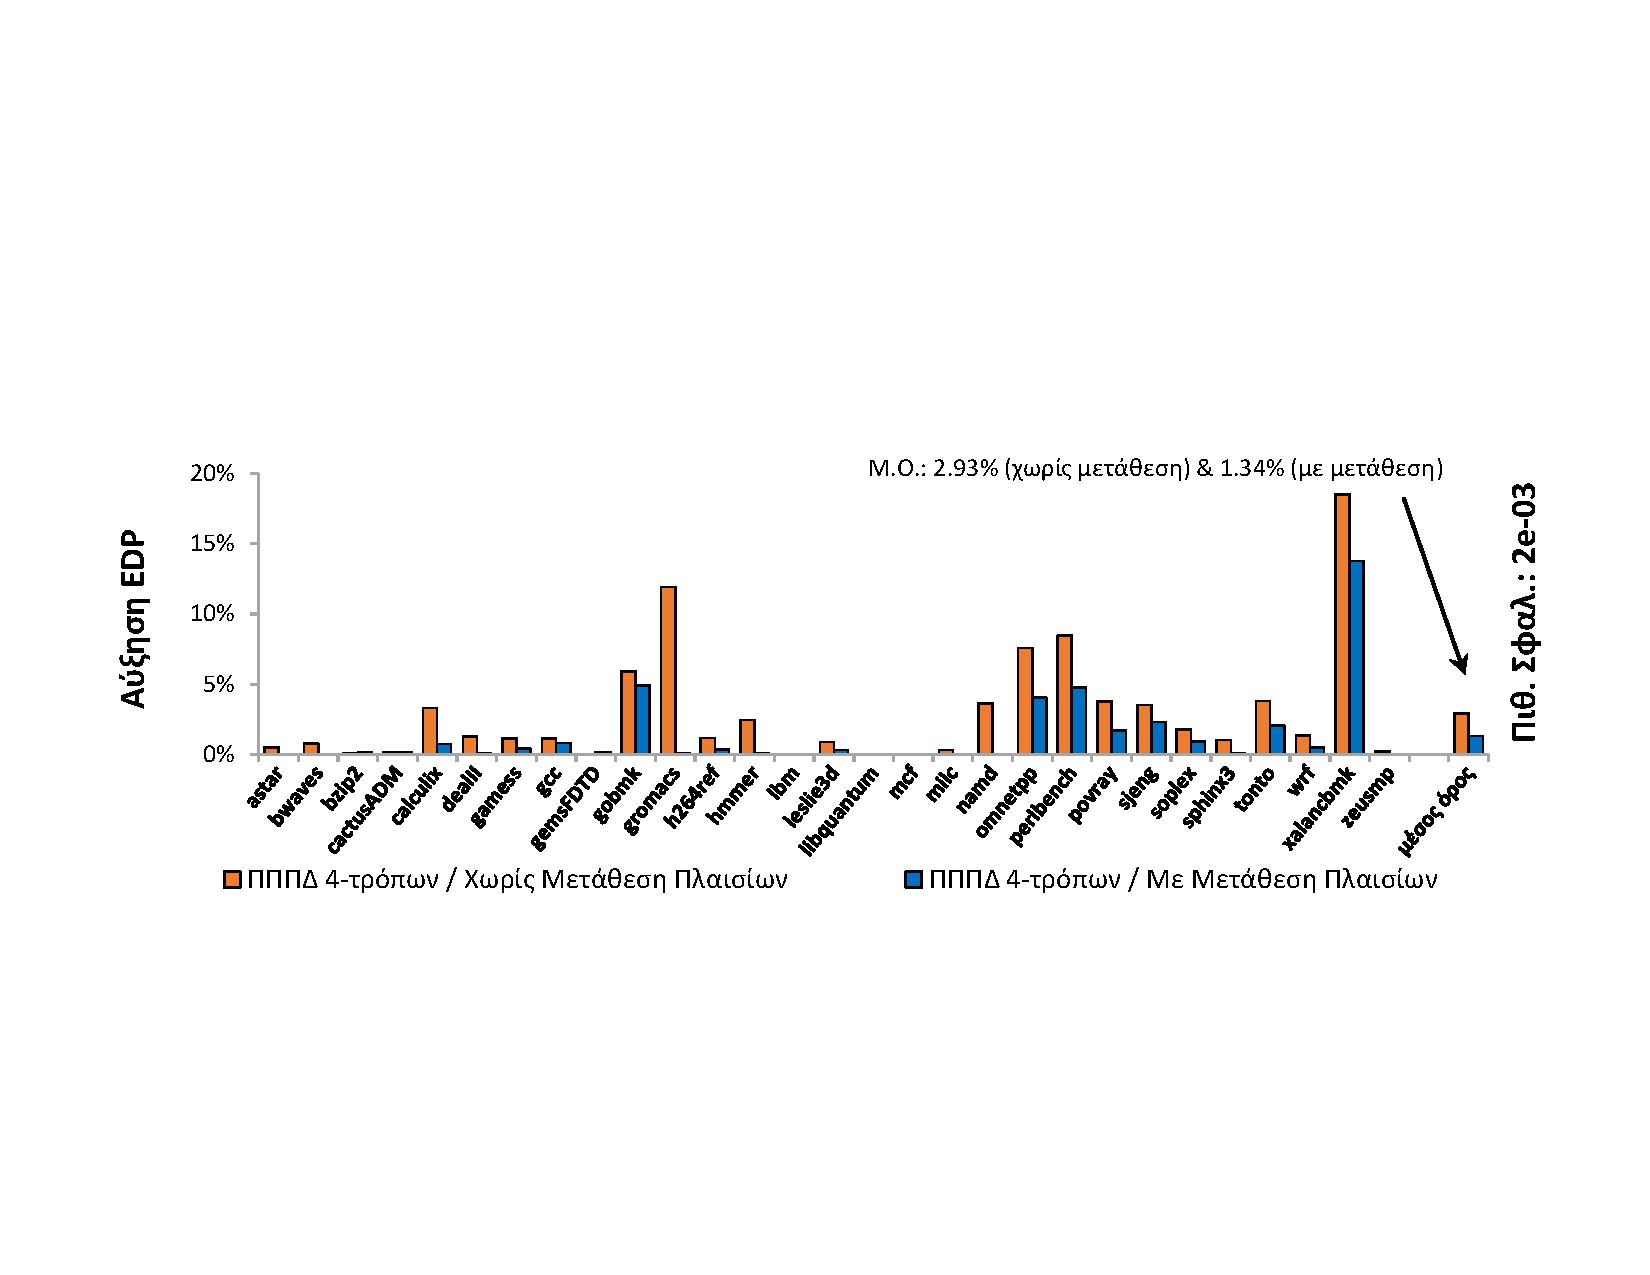
\includegraphics[width=\linewidth, trim=2cm 6.4cm 1.6cm 7.7cm, clip=true]{\resultsDIR/chap6_BTB_edp_serial_w4_pfail1.pdf}}
        \caption{Πιθανότητα Σφάλματος 1}
        \label{fig:chap6_serial_4way_pail1_edp}
    \end{subfigure}
    
    \begin{subfigure}[t]{\textwidth}
        \centering
        \fbox{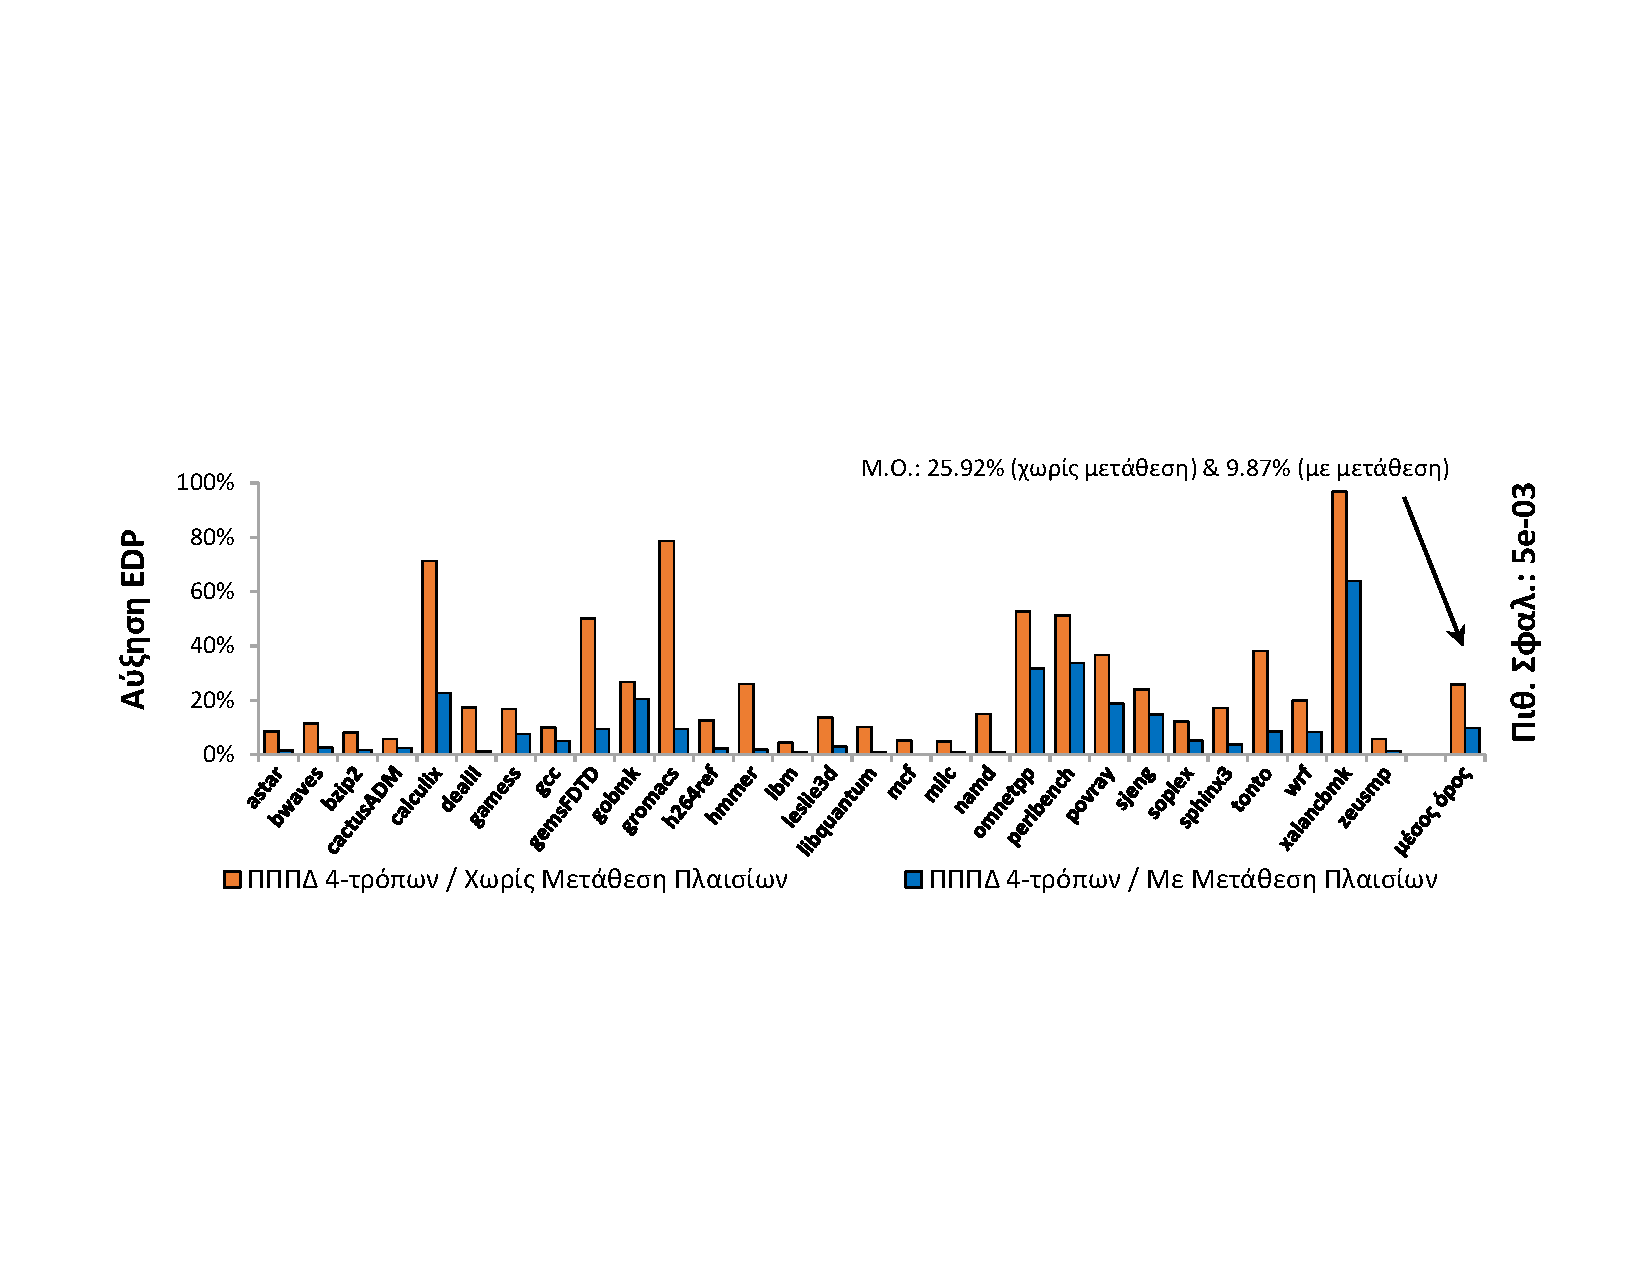
\includegraphics[width=\linewidth, trim=2cm 6.4cm 1.6cm 7.7cm, clip=true]{\resultsDIR/chap6_BTB_edp_serial_w4_pfail2.pdf}}
        \caption{Πιθανότητα Σφάλματος 2}
        \label{fig:chap6_serial_4way_pail2_edp}
    \end{subfigure}
    \caption{Αποτελέσματα με χρήση του σειριακού αλγορίθμου - (4-τρόπων ΠΠΠΔ)}
    \label{fig:chap6_serial_4way_edp}
\end{figure}

%----------------------------------------------------------%

\subsection{Αποτελέσματα Ενισχυμένου Παράλληλου Μοντέλου}
\label{chap6_mcpatParallelAlgResults}

Όπως αποδείχθηκε, η χρήση του παράλληλου αλγορίθμου δεν προσφέρει καλύτερα αποτελέσματα στην απόδοση από αυτή του σειριακού και επομένως δεν αναμένονται καλύτερα αποτελέσματα στην κατανάλωση. Παρόλα αυτά, αξίζει να γίνει η μελέτη των αντίστοιχων αποτελεσμάτων και αυτής της λύσης όταν η οργάνωση είναι 4-τρόπων. Τα αποτελέσματά της παρουσιάζονται στο Σχήμα \ref{fig:chap6_parallel_4way_edp}.
\par
Όταν η πιθανότητα σφάλματος είναι $\expnum{2}$ (γράφημα \ref{fig:chap6_parallel_4way_pail1_edp}) η αύξηση του \edp ελαττώνεται κατά μέσο όρο από $2.93\%$ σε $1.57\%$. Επομένως η επαναφορά της κατανάλωσης είναι $46\%$, από $54\%$ που επέφερε η χρήση του σειριακού αλγορίθμου. Αντίστοιχα, για την πιθανότητα σφάλματος $\expnum{5}$ (γράφημα \ref{fig:chap6_parallel_4way_pail2_edp}) η αύξηση του \edp ελαττώνεται κατά μέσο όρο από $25.92\%$ σε $11.47\%$. Σε αυτή την περίπτωση η επαναφορά είναι $56\%$, από $62\%$ που επέφερε η χρήση του σειριακού αλγορίθμου.

\begin{figure}[!t]
    \centering
    \begin{subfigure}[t]{\textwidth}
        \centering
        \fbox{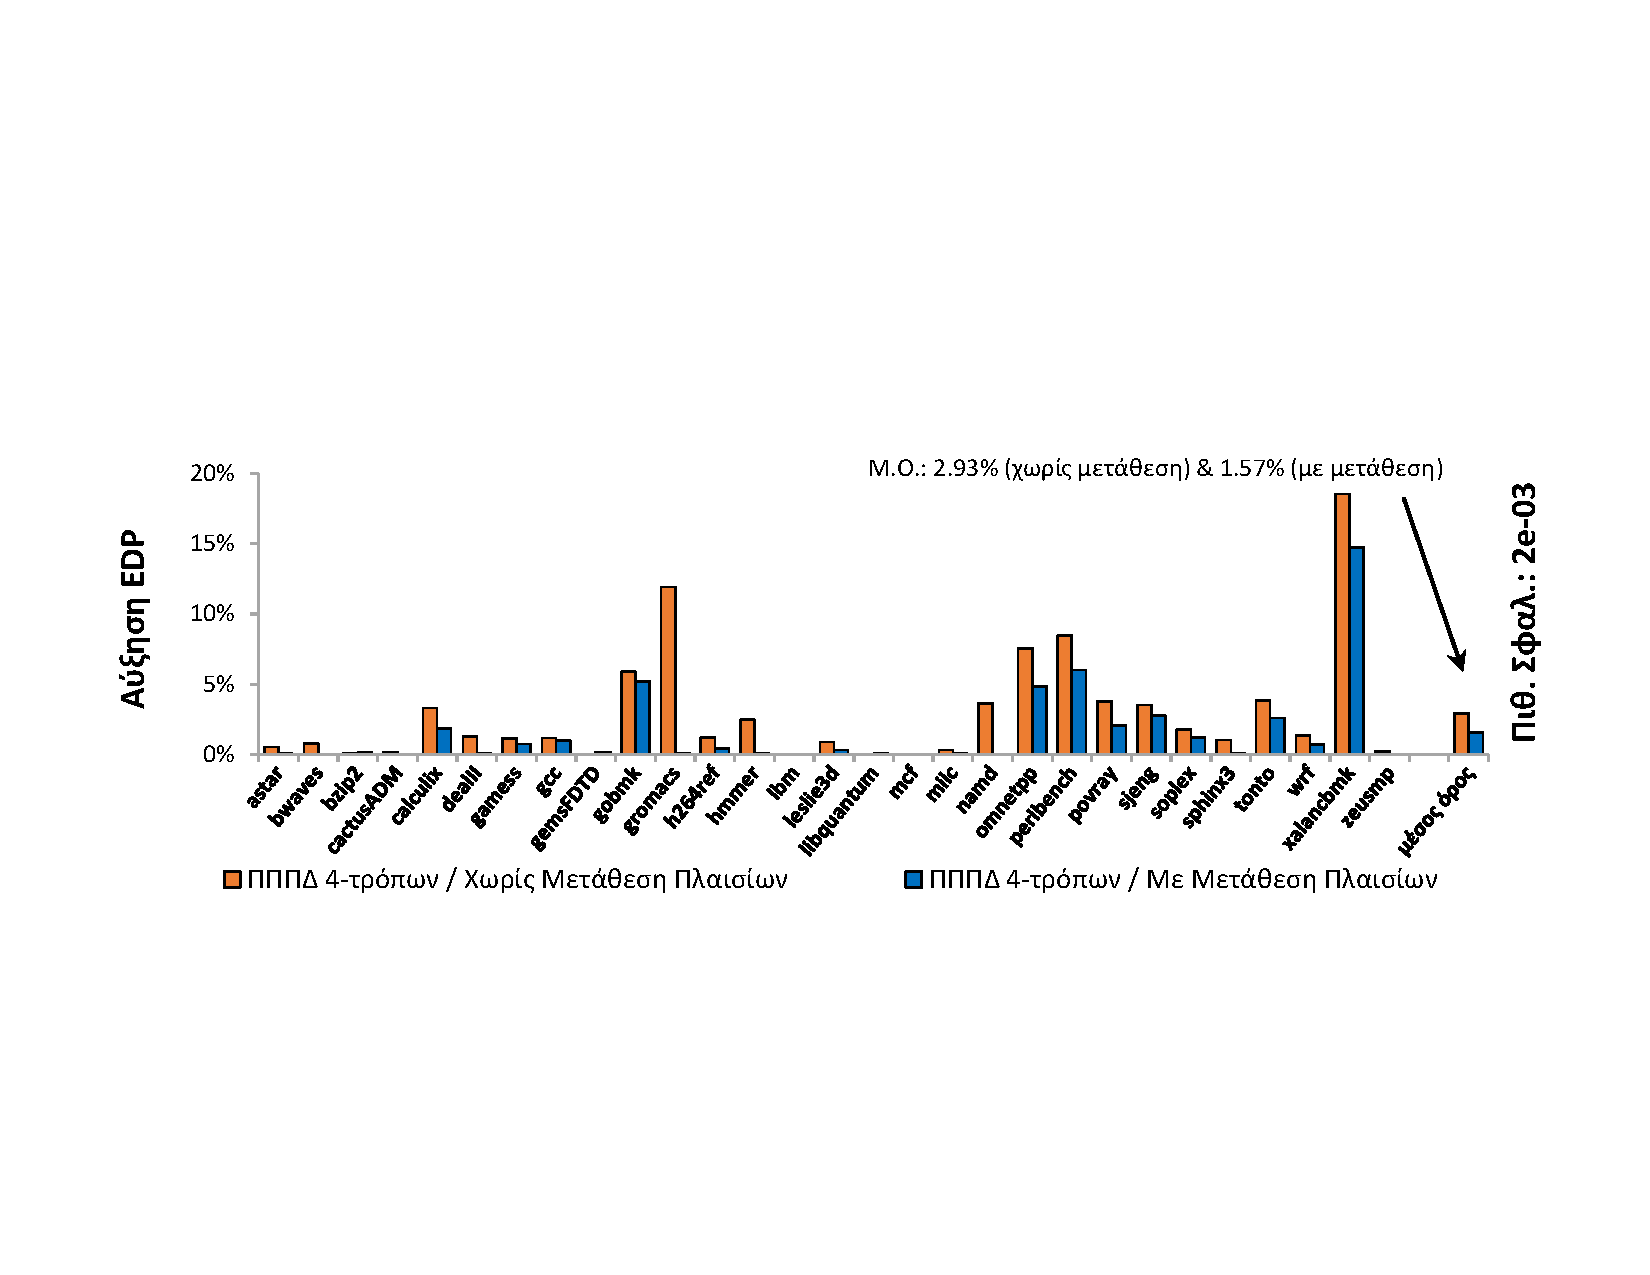
\includegraphics[width=\linewidth, trim=2cm 6.4cm 1.6cm 7.7cm, clip=true]{\resultsDIR/chap6_BTB_edp_parallel_w4_pfail1.pdf}}
        \caption{Πιθανότητα Σφάλματος 1}
        \label{fig:chap6_parallel_4way_pail1_edp}
    \end{subfigure}
    
    \begin{subfigure}[t]{\textwidth}
        \centering
        \fbox{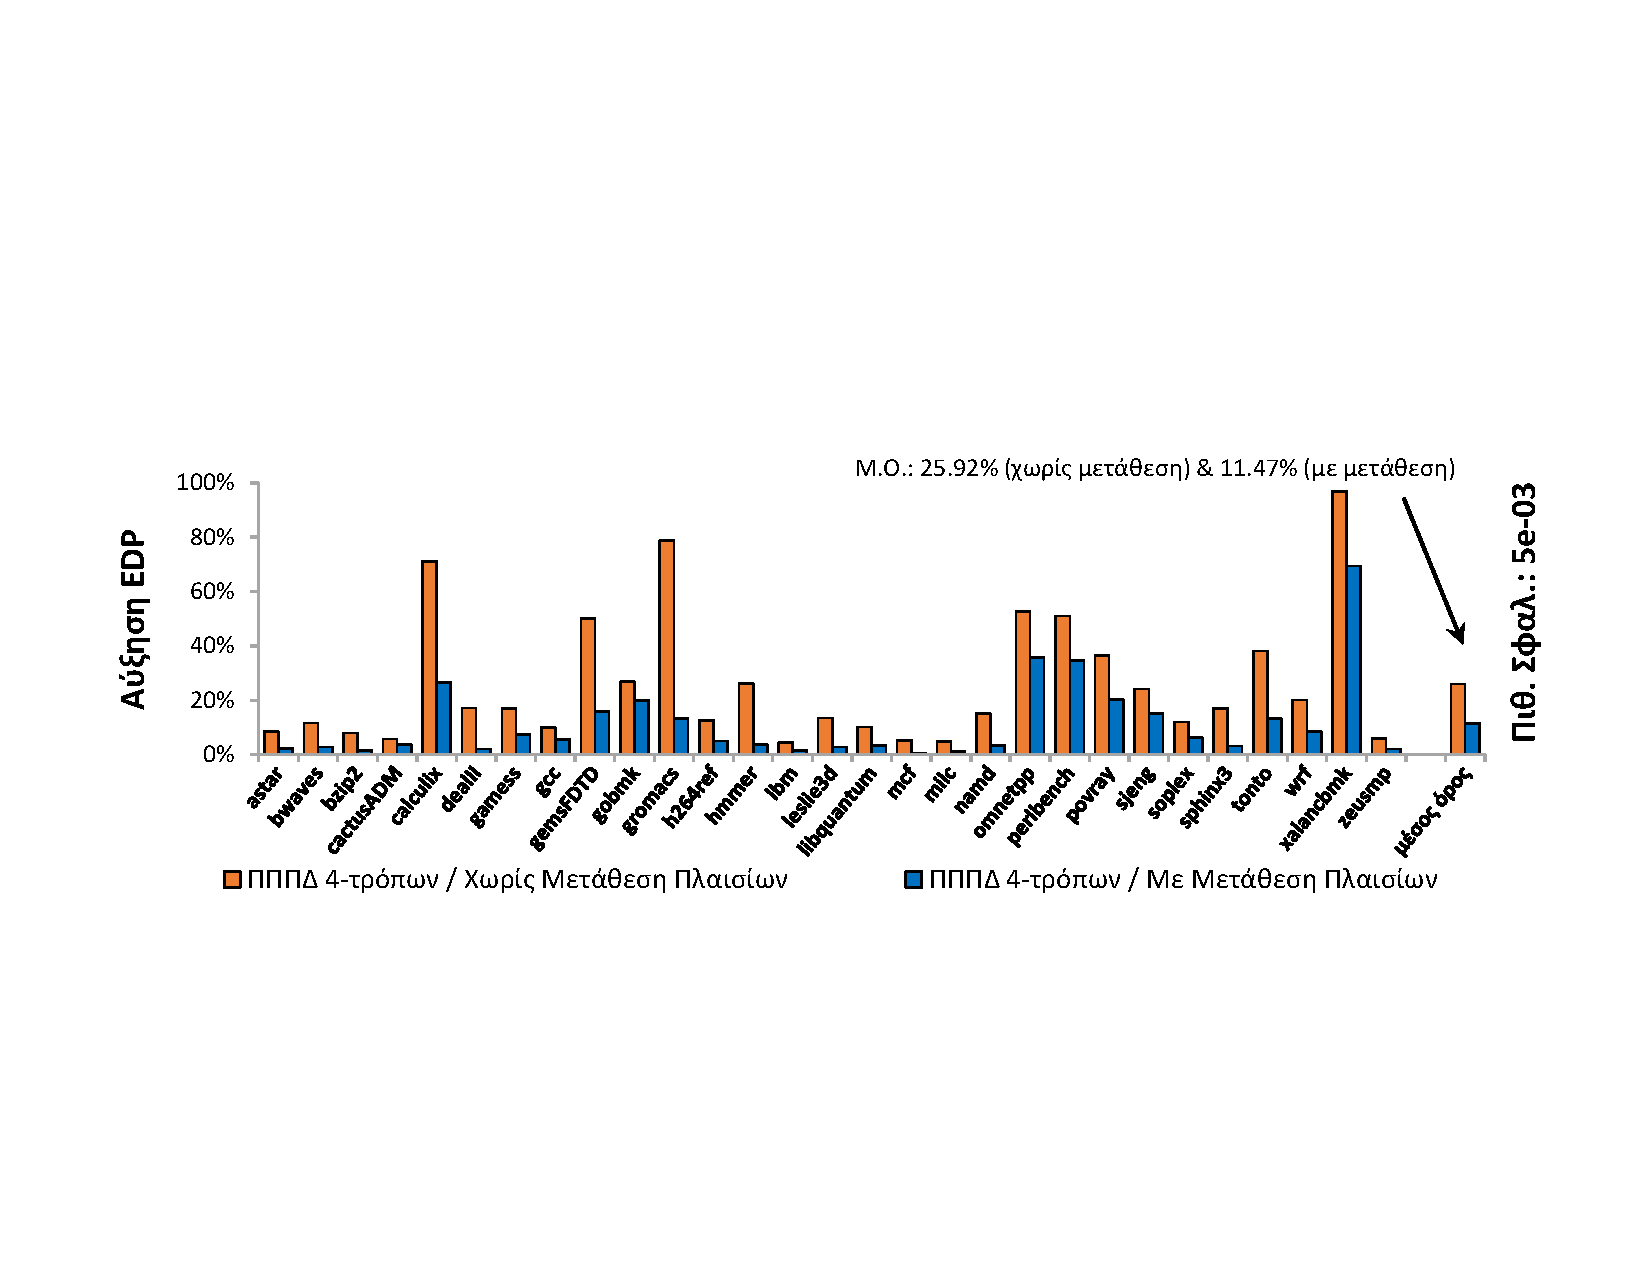
\includegraphics[width=\linewidth, trim=2cm 6.4cm 1.6cm 7.7cm, clip=true]{\resultsDIR/chap6_BTB_edp_parallel_w4_pfail2.pdf}}
        \caption{Πιθανότητα Σφάλματος 2}
        \label{fig:chap6_parallel_4way_pail2_edp}
    \end{subfigure}
    \caption{Αποτελέσματα με χρήση του παράλληλου αλγορίθμου}
    \label{fig:chap6_parallel_4way_edp}
\end{figure}

%----------------------------------------------------------%

\subsection{Αποτελέσματα Βελτιστοποιημένου Σειριακού Μοντέλου}
\label{chap6_mcpatOptimizedSerialAlgResults}

Τελευταίο τμήμα της αξιολόγησης αποτελεί η σύγκριση μεταξύ των καταναλώσεων όταν δεν χρησιμοποιείται κάποια μέθοδος για την αντιμετώπιση των σφαλμάτων του Πίνακα Πρόβλεψης Προορισμού Διακλάδωσης (βασικό μοντέλο) και όταν εφαρμόζεται η τεχνική της λογικής μετάθεσης πλαισίων με χρήση πολλαπλών καταχωρητών ανά τμήμα (βελτιστοποιημένο μοντέλο). Όπως έχει ήδη αναφερθεί, η αύξηση του πλήθους καταχωρητών μπορεί να προκαλέσει μικρή αύξηση στην κατανάλωση του Πίνακα Πρόβλεψης Προορισμού Διακλάδωσης. Παρόλα αυτά, όπως αποδεικνύεται στην παρούσα υποενότητα η συνολική κατανάλωση για την εκτέλεση ενός προγράμματος μειώνεται δραματικά με τη χρήση αυτής της βελτιστοποιημένης τεχνικής, εξαιτίας της δραστικής μείωσης του χρόνου εκτέλεσης των προγραμμάτων.
\par
Στην παρούσα μελέτη θεωρήθηκε πως γίνεται χρήση του πρώτου τρόπου υλοποίησης στο υλικό (Σχήμα \ref{fig:chap5_permutation_impl_v1}), για οργανώσεις 2 και 4-τρόπων με διάσπαση σε 64 και 4 υποτμήματα αντίστοιχα. Τα αποτελέσματα της μελέτης των δύο οργανώσεων παρουσιάζονται στα Σχήματα \ref{fig:chap6_optimized_serial_2way_edp} και \ref{fig:chap6_optimized_serial_4way_edp}.

\begin{figure}[!t]
    \centering
    \begin{subfigure}[t]{\textwidth}
        \centering
        \fbox{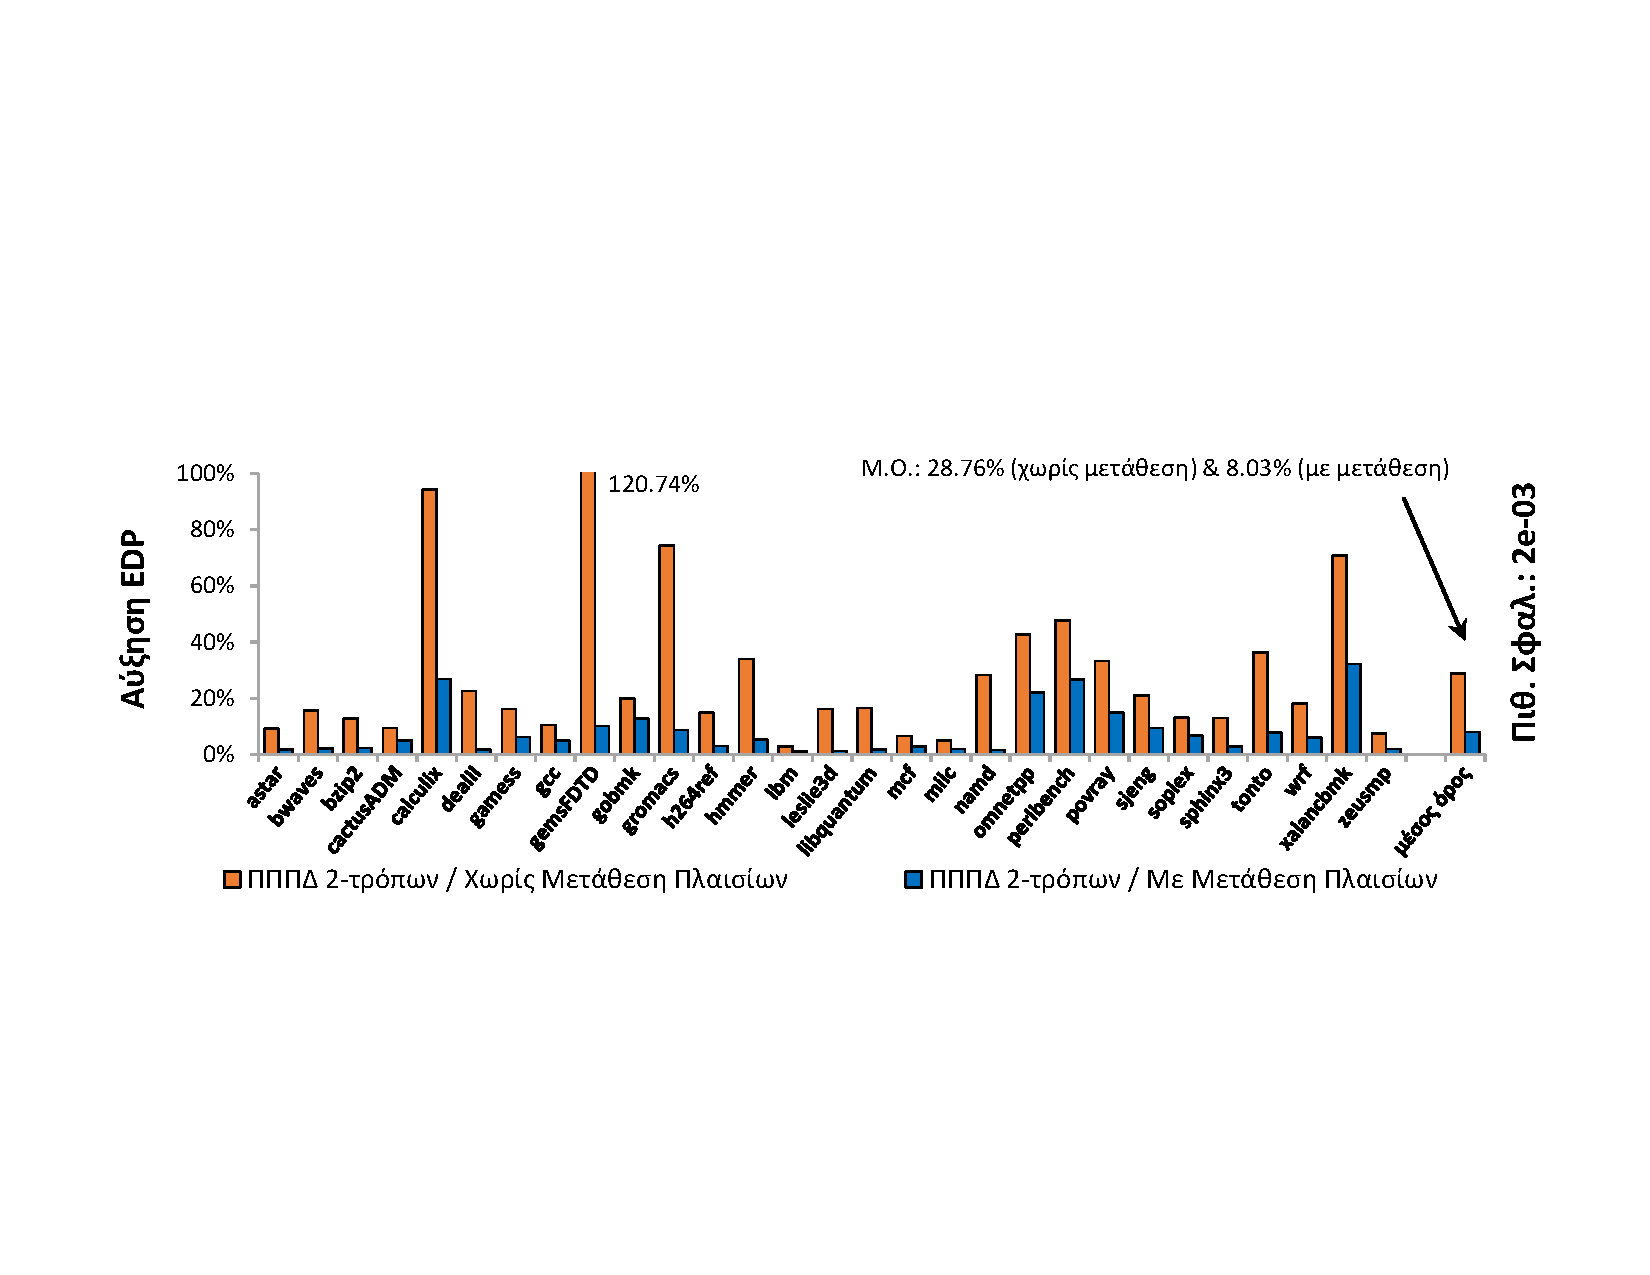
\includegraphics[width=\linewidth, trim=2cm 6.4cm 1.6cm 7.7cm, clip=true]{\resultsDIR/chap6_BTB_edp_optimized_serial_w2_pfail1.pdf}}
        \caption{Πιθανότητα Σφάλματος 1}
        \label{fig:chap6_optimized_serial_2way_pail1_edp}
    \end{subfigure}
    
    \begin{subfigure}[t]{\textwidth}
        \centering
        \fbox{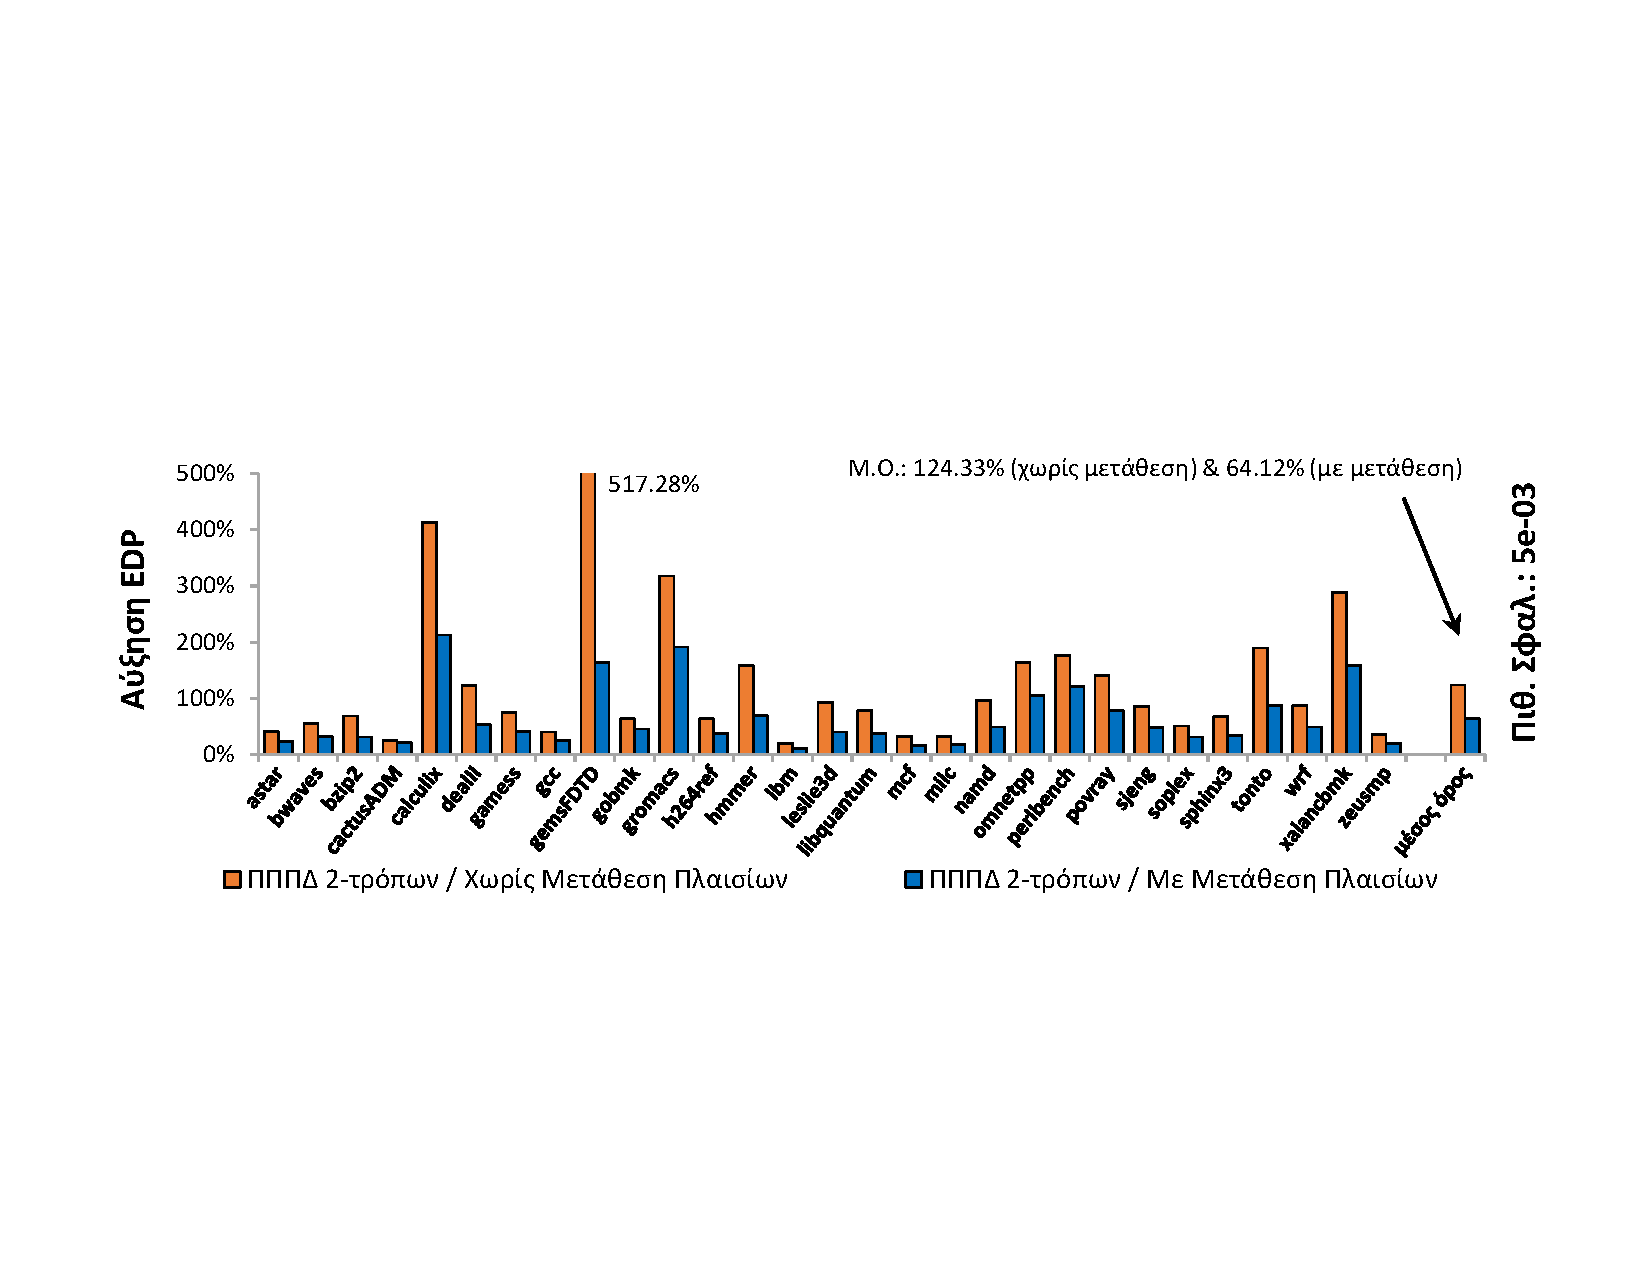
\includegraphics[width=\linewidth, trim=2cm 6.4cm 1.6cm 7.7cm, clip=true]{\resultsDIR/chap6_BTB_edp_optimized_serial_w2_pfail2.pdf}}
        \caption{Πιθανότητα Σφάλματος 2}
        \label{fig:chap6_optimized_serial_2way_pail2_edp}
    \end{subfigure}
    
    \caption{Αποτελέσματα με διάσπαση σε υποτμήματα και χρήση του σειριακού αλγορίθμου (2-τρόπων ΠΠΠΔ)}
    \label{fig:chap6_optimized_serial_2way_edp}
\end{figure}

Στην περίπτωση της οργάνωσης 2-τρόπων και πιθανότητας σφάλματος $\expnum{2}$ (γράφημα \ref{fig:chap6_optimized_serial_2way_pail1_edp}) η αύξηση του \edp ελαττώνεται κατά μέσο όρο από $28.76\%$ σε $8.03\%$. Επομένως η επαναφορά της κατανάλωσης είναι $72\%$, από $51\%$ που προσέφερε η χρήση ενός μόνο καταχωρητή ανά τμήμα (ενισχυμένο σειριακό μοντέλο). Όπως και στην περίπτωση της χρήσης ενός Καταχωρητή Διαμόρφωσης, το μετροπρόγραμμα \en{gemsFDTD} παρουσιάζει την εντονότερη βελτίωση, με την αύξηση της κατανάλωσης να μεταβάλλεται από $120.74\%$ σε μόλις $10.15\%$ (επαναφορά κατά $91\%$).
\par
Αντίστοιχα, όταν η πιθανότητα σφάλματος ανεβαίνει σε $\expnum{5}$ (γράφημα \ref{fig:chap6_optimized_serial_2way_pail2_edp}) η αύξηση του \edp ελαττώνεται κατά μέσο όρο από $124.33\%$ σε $64.12\%$. Επομένως η επαναφορά της κατανάλωσης είναι $48\%$, από $16\%$ που ήταν με τη χρήση ενός μόνο καταχωρητή. Για ακόμη μία φορά το μετροπρόγραμμα \en{gemsFDTD} παρουσιάζεται τη σημαντικότερη βελτίωση καθώς η αύξηση της κατανάλωσης μεταβάλλεται από $517.28\%$ σε $164.19\%$ (επαναφορά κατά $68\%$).
\par
Η επαναφορά της κατανάλωσης γίνεται ακόμη μεγαλύτερη στην περίπτωση της οργάνωσης 4-τρόπων συνόλου συσχέτισης και πιθανότητας σφάλματος $\expnum{5}$, όπως παρουσιάζεται στο Σχήμα \ref{fig:chap6_optimized_serial_4way_edp}. Όπως αναγράφεται, η αύξηση του \edp ελαττώνεται κατά μέσο όρο από $25.92\%$ σε $6.19\%$. Επομένως η επαναφορά της κατανάλωσης είναι $76\%$, από $62\%$ που ήταν με τη χρήση ενός καταχωρητή ανά τμήμα. Σε αυτή την περίπτωση στο μετροπρόγραμμα \en{gromacs}, το οποίο εμφανίζει τη μεγαλύτερη βελτίωση, η αύξηση της κατανάλωσης μεταβάλλεται από $78.69\%$ σε μόλις $0.61\%$ (επαναφορά κατά $99\%$).

\begin{figure}[!t]
    \centering
    \fbox{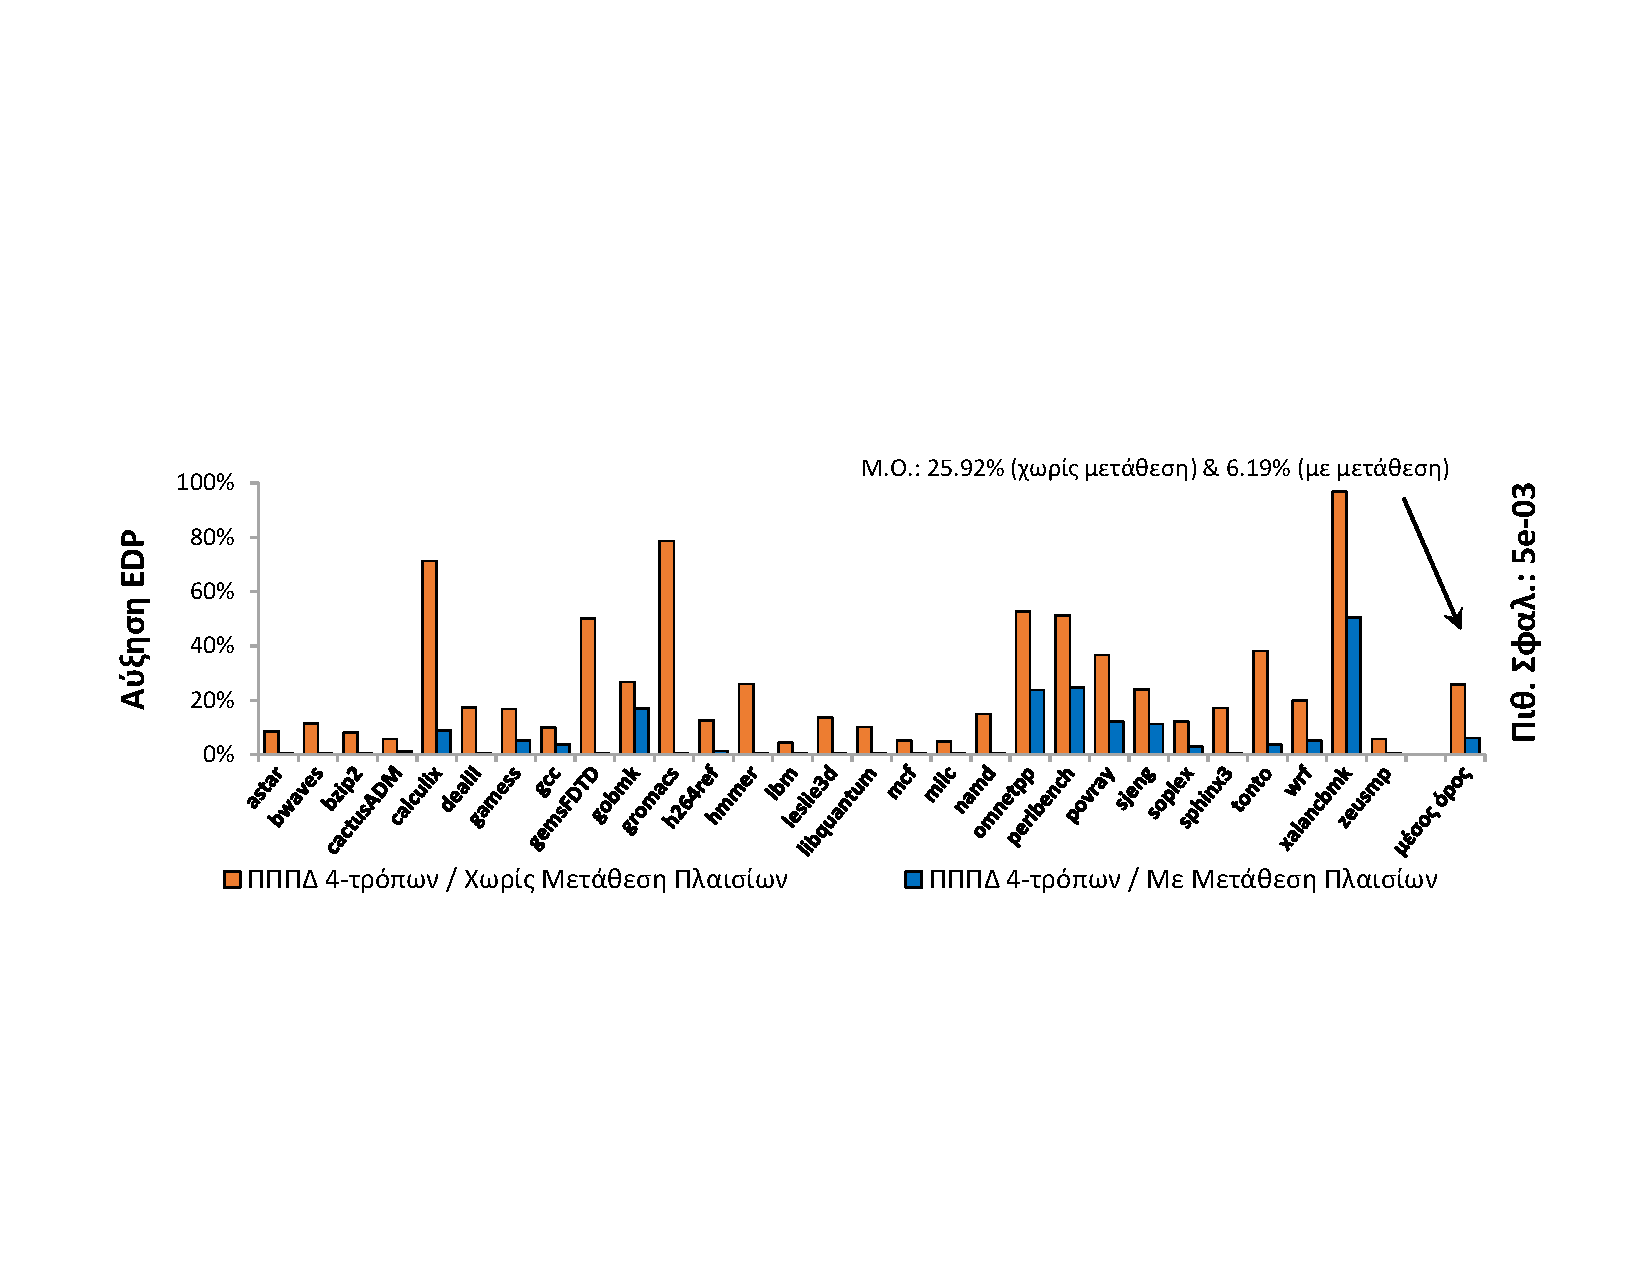
\includegraphics[width=\linewidth, trim=2cm 6.4cm 1.6cm 7.7cm, clip=true]{\resultsDIR/chap6_BTB_edp_optimized_serial_w4_pfail2.pdf}}
    \caption{Αποτελέσματα με διάσπαση σε υποτμήματα και χρήση του σειριακού αλγορίθμου (4-τρόπων ΠΠΠΔ / Πιθανότητα Σφάλματος 2)}
    \label{fig:chap6_optimized_serial_4way_edp}
\end{figure}

%----------------------------------------------------------%

\section{Συμπεράσματα Αξιολόγησης}

Σκοπός της αξιολόγησης τόσο στο κομμάτι του χρόνου εκτέλεσης όσο και της κατανάλωσης, ήταν η ανάδειξης της προσφοράς της προτεινόμενης τεχνικής στη λειτουργία του υπερβαθμωτού επεξεργαστή όταν η τάση λειτουργίας που εφαρμόζεται σε αυτόν μειώνεται με σκοπό τη μείωση της συνολικής απαιτούμενης ενέργειας. Με βάση τα αποτελέσματα που παρουσιάστηκαν στις Ενότητες \ref{chap6_gem5Results} και \ref{chap6_mcpatResults} κατέστη σαφές πως για την κάλυψη μεγάλου εύρους τάσεων λειτουργίας, η χρήση της βελτιστοποιημένης μεθόδου αποτελεί την καλύτερη επιλογή μεταξύ των προτεινόμενων λύσεων. Στον Πίνακα \ref{tab:chap6_finalResults} παρουσιάζονται τα συγκεντρωτικά αποτελέσματα πριν και μετά την εφαρμογή της βέλτιστης τεχνικής λογικής μετάθεσης πλαισίων (μείωση \ipc / αύξηση \edp).

\begin{table}[!b]
    \centering
    \begin{tabularx}{\textwidth}{>{\centering\arraybackslash}c >{\centering\arraybackslash}X >{\centering\arraybackslash}X}
        \Xhline{4\arrayrulewidth}
        \textbf{Οργάνωση ΠΠΠΔ}          & \textbf{Μείωση \ipc}  & \textbf{Αύξηση \edp} \\
        \textbf{(Πιθανότητα Σφάλματος)} & \textbf{(Πριν/Μετά)}  & \textbf{(Πριν/Μετά)} \\
        \hline
        {2-τρόπων ($\expnum{2}$)}       & {$8.6\%$ / $2.7\%$}   & {$28.8\%$ / $8.0\%$} \\
        {2-τρόπων ($\expnum{5}$)}       & {$25.5\%$ / $15.9\%$} & {$124.3\%$ / $64.1\%$} \\
        {4-τρόπων ($\expnum{2}$)}       & {$1.2\%$ / $0.6\%$}  & {$2.9\%$ / $1.3\%$} \\
        {4-τρόπων ($\expnum{5}$)}       & {$8.1\%$ / $2.4\%$}   & {$25.9\%$ / $6.2\%$} \\
        \Xhline{4\arrayrulewidth}
    \end{tabularx}
    \caption{Αποτελέσματα πριν και μετά την εφαρμογή της βέλτιστης τεχνικής λογικής μετάθεσης πλαισίων}
    \label{tab:chap6_finalResults}
\end{table}

%----------------------------------------------------------%
